\documentclass{Configuration_Files/PoliMi3i_thesis}

%------------------------------------------------------------------------------
%	REQUIRED PACKAGES AND  CONFIGURATIONS
%------------------------------------------------------------------------------

% CONFIGURATIONS
\usepackage{parskip} % For paragraph layout
\usepackage{setspace} % For using single or double spacing
\usepackage{emptypage} % To insert empty pages
\usepackage{multicol} % To write in multiple columns (executive summary)
\usepackage{minted}
\setlength\columnsep{15pt} % Column separation in executive summary
\setlength\parindent{0pt} % Indentation
\raggedbottom  

% PACKAGES FOR TITLES
\usepackage{titlesec}
% \titlespacing{\section}{left spacing}{before spacing}{after spacing}
\titlespacing{\section}{0pt}{3.3ex}{2ex}
\titlespacing{\subsection}{0pt}{3.3ex}{1.65ex}
\titlespacing{\subsubsection}{0pt}{3.3ex}{1ex}
\usepackage{color}

% PACKAGES FOR LANGUAGE AND FONT
\usepackage[english]{babel} % The document is in English  
\usepackage[utf8]{inputenc} % UTF8 encoding
\usepackage[T1]{fontenc} % Font encoding
\usepackage[11pt]{moresize} % Big fonts

% PACKAGES FOR IMAGES
\usepackage{graphicx}
\usepackage{transparent} % Enables transparent images
\usepackage{eso-pic} % For the background picture on the title page
\usepackage{subfig} % Numbered and caption subfigures using \subfloat.
\usepackage{tikz} % A package for high-quality hand-made figures.
\usetikzlibrary{}
\graphicspath{{./Images/}} % Directory of the images
\usepackage{caption} % Coloured captions
\usepackage{xcolor} % Coloured captions
\usepackage{amsthm,thmtools,xcolor} % Coloured "Theorem"
\usepackage{float}

% STANDARD MATH PACKAGES
\usepackage{amsmath}
\usepackage{amsthm}
\usepackage{amssymb}
\usepackage{amsfonts}
\usepackage{bm}
\usepackage[overload]{empheq} % For braced-style systems of equations.
\usepackage{fix-cm} % To override original LaTeX restrictions on sizes

% PACKAGES FOR TABLES
\usepackage{tabularx}
\usepackage{longtable} % Tables that can span several pages
\usepackage{colortbl}

% PACKAGES FOR ALGORITHMS (PSEUDO-CODE)
\usepackage{algorithm}
\usepackage{algorithmic}

% PACKAGES FOR REFERENCES & BIBLIOGRAPHY
\usepackage[colorlinks=true,linkcolor=black,anchorcolor=black,citecolor=black,filecolor=black,menucolor=black,runcolor=black,urlcolor=black]{hyperref} % Adds clickable links at references
\usepackage{cleveref}
\usepackage[square, numbers, sort&compress]{natbib} % Square brackets, citing references with numbers, citations sorted by appearance in the text and compressed
\bibliographystyle{abbrvnat} % You may use a different style adapted to your field

% OTHER PACKAGES
\usepackage{pdfpages} % To include a pdf file
\usepackage{afterpage}
\usepackage{lipsum} % DUMMY PACKAGE
\usepackage{fancyhdr} % For the headers
\fancyhf{}

% Input of configuration file. Do not change config.tex file unless you really know what you are doing. 
% Define blue color typical of polimi
\definecolor{bluepoli}{cmyk}{0.4,0.1,0,0.4}

% Custom theorem environments
\declaretheoremstyle[
  headfont=\color{bluepoli}\normalfont\bfseries,
  bodyfont=\color{black}\normalfont\itshape,
]{colored}

% Set-up caption colors
\captionsetup[figure]{labelfont={color=bluepoli}} % Set colour of the captions
% \captionsetup[table]{labelfont={color=bluepoli}} % Set colour of the captions
% \captionsetup[algorithm]{labelfont={color=bluepoli}} % Set colour of the captions

\theoremstyle{colored}
\newtheorem{theorem}{Theorem}[chapter]
\newtheorem{proposition}{Proposition}[chapter]

% Enhances the features of the standard "table" and "tabular" environments.
\newcommand\T{\rule{0pt}{2.6ex}}
\newcommand\B{\rule[-1.2ex]{0pt}{0pt}}

% Pseudo-code algorithm descriptions.
\newcounter{algsubstate}
\renewcommand{\thealgsubstate}{\alph{algsubstate}}
\newenvironment{algsubstates}
  {\setcounter{algsubstate}{0}%
   \renewcommand{\STATE}{%
     \stepcounter{algsubstate}%
     \Statex {\small\thealgsubstate:}\space}}
  {}

% New font size
\newcommand\numfontsize{\@setfontsize\Huge{200}{60}}

% Title format: chapter
\titleformat{\chapter}[hang]{
\fontsize{50}{20}\selectfont\bfseries\filright}{\textcolor{bluepoli} \thechapter\hsp\hspace{2mm}\textcolor{bluepoli}{|   }\hsp}{0pt}{\huge\bfseries \textcolor{bluepoli}
}

% Title format: section
\titleformat{\section}
{\color{bluepoli}\normalfont\Large\bfseries}
{\color{bluepoli}\thesection.}{1em}{}

% Title format: subsection
\titleformat{\subsection}
{\color{bluepoli}\normalfont\large\bfseries}
{\color{bluepoli}\thesubsection.}{1em}{}

% Title format: subsubsection
\titleformat{\subsubsection}
{\color{bluepoli}\normalfont\large\bfseries}
{\color{bluepoli}\thesubsubsection.}{1em}{}

% Shortening for setting no horizontal-spacing
\newcommand{\hsp}{\hspace{0pt}}

\makeatletter
% Renewcommand: cleardoublepage including the background pic
\renewcommand*\cleardoublepage{%
  \clearpage\if@twoside\ifodd\c@page\else
  \null
  \AddToShipoutPicture*{\BackgroundPic}
  \thispagestyle{empty}%
  \newpage
  \if@twocolumn\hbox{}\newpage\fi\fi\fi}
\makeatother

%For correctly numbering algorithms
\numberwithin{algorithm}{chapter}

%----------------------------------------------------------------------------
%	NEW COMMANDS DEFINED
%----------------------------------------------------------------------------

% EXAMPLES OF NEW COMMANDS
\newcommand{\bea}{\begin{eqnarray}} % Shortcut for equation arrays
\newcommand{\eea}{\end{eqnarray}}
\newcommand{\e}[1]{\times 10^{#1}}  % Powers of 10 notation

%----------------------------------------------------------------------------
%	ADD YOUR PACKAGES (be careful of package interaction)
%----------------------------------------------------------------------------

%----------------------------------------------------------------------------
%	ADD YOUR DEFINITIONS AND COMMANDS (be careful of existing commands)
%----------------------------------------------------------------------------

%----------------------------------------------------------------------------
%	BEGIN OF YOUR DOCUMENT
%----------------------------------------------------------------------------

\begin{document}

\fancypagestyle{plain}{%
\fancyhf{} % Clear all header and footer fields
\fancyhead[RO,RE]{\thepage} %RO=right odd, RE=right even
\renewcommand{\headrulewidth}{0pt}
\renewcommand{\footrulewidth}{0pt}}

%----------------------------------------------------------------------------
%	TITLE PAGE
%----------------------------------------------------------------------------

\pagestyle{empty} % No page numbers
\frontmatter % Use roman page numbering style (i, ii, iii, iv...) for the preamble pages

\puttitle{
	title=Implementation of a Key Management Entity for Quantum Key Distribution, % Title of the thesis
	name=Nicolò Sala, % Author Name and Surname
	course=Computer Science Engineering - Ingegneria Informatica, % Study Programme (in Italian)
	ID  = 945898,  % Student ID number (numero di matricola)
	advisor= Prof. Paolo Martelli, % Supervisor name
	coadvisor={Alberto Gatto, Marco Brunero}, % Co-Supervisor name, remove this line if there is none
	academicyear={2021-22},  % Academic Year
} % These info will be put into your Title page 

%----------------------------------------------------------------------------
%	PREAMBLE PAGES: ABSTRACT (inglese e italiano), EXECUTIVE SUMMARY
%----------------------------------------------------------------------------
\startpreamble
\setcounter{page}{1} % Set page counter to 1

% ABSTRACT IN ENGLISH
\chapter*{Abstract} 
The Internet requires the ability to exchange secret keys through a public communication channel. Each key is then used to encrypt confidential messages between two entities.

The current protocols for exchanging secret keys are based on mathematical problems that are extremely hard to solve, requiring a time of computation too long also for the most powerful today's classical computer.

However, the development of quantum computers will soon make it easy to tackle such problems, resulting in a lack of security in our communications.

Today's most promising solution is Quantum Key Distribution (QKD). It allows unconditional secure sharing of secrets based on quantum mechanics' fundamental principles.

The secret bit sequences produced through QKD have a length that cannot be determined a priori, while applications often need a key with a predetermined length. Furthermore, once produced via QKD, the bit sequence must be made available to applications in an equally secure manner.

This document describes the implementation of a Key Management Entity (KME), the software dedicated to creating secret keys of fixed length, starting from the bits shared securely through QKD.

After describing the evolution of the problem of sharing secrets in a public channel showing QKD as a solution, we move on to the description of how KME works. After that, the details of the proposed implementation are analyzed to finally arrive at the interaction of the KME with currently available quantum modules.


\textbf{Keywords}: Quantum Key Distribution, Key Management Entity

% ABSTRACT IN ITALIAN
\chapter*{Abstract in lingua italiana}
Internet richiede la capacità di scambiare chiavi segrete attraverso un canale di comunicazione pubblico. Ogni chiave è poi utilizzata per cifrare messaggi confidenziali tra due entità.

Gli attuali protocolli informatici per lo scambio di chiavi segrete sono basati su problemi di matematica molto difficili da risolvere, poiché richiedono un tempo di elaborazione troppo lungo anche per il computer elettronico più potente ad oggi.

Tuttavia, lo sviluppo di computer quantistici renderà presto semplice la risoluzione di tali problemi, portando di conseguenza a una mancanza di sicurezza nelle nostre comunicazioni.

La soluzione più promettente al giorno d'oggi è la Quantum Key Distribution (QKD), la quale consente di condividere segreti in modo incondizionatamente sicuro, basandosi sui principi fondamentali della meccanica quantistica.

Le sequenze di bit segrete prodotte attraverso QKD hanno una lunghezza non determinabile a priori, mentre le applicazioni spesso necessitano di una chiave di lunghezza prefissata. Inoltre, la sequenza di bit, una volta prodotta tramite QKD, deve essere messa a disposizione delle applicazioni in maniera altrettanto sicura.

Questo documento descrive l'implementazione di una Key Management Entity (KME), il software dedito alla creazione di chiavi segrete di lunghezza fissata, a partire dai bit condivisi in maniera sicura tramite QKD.

Dopo aver descritto l'evoluzione del problema di condivisione di segreti in un canale pubblico, mostrando QKD come soluzione, si passa alla descrizione del funzionamento della KME. Dopodiché, si analizzano i dettagli dell'implementazione proposta, per giungere infine all'interazione della KME con moduli quantistici attualmente disponibili.

\textbf{Parole chiave}: Quantum Key Distribution, Key Management Entity

%----------------------------------------------------------------------------
%	LIST OF CONTENTS/FIGURES/TABLES/SYMBOLS
%----------------------------------------------------------------------------

% TABLE OF CONTENTS
\thispagestyle{empty}
\tableofcontents % Table of contents 
\thispagestyle{empty}
\cleardoublepage

%-------------------------------------------------------------------------
%	THESIS MAIN TEXT
%-------------------------------------------------------------------------
% In the main text of your thesis you can write the chapters in two different ways:
%
%(1) As presented in this template you can write:
%    \chapter{Title of the chapter}
%    *body of the chapter*
%
%(2) You can write your chapter in a separated .tex file and then include it in the main file with the following command:
%    \chapter{Title of the chapter}
%    \input{chapter_file.tex}
%
% Especially for long thesis, we recommend you the second option.

\addtocontents{toc}{\vspace{2em}} % Add a gap in the Contents, for aesthetics
\mainmatter % Begin numeric (1,2,3...) page numbering

% --------------------------------------------------------------------------
% NUMBERED CHAPTERS % Regular chapters following
% --------------------------------------------------------------------------

\chapter*{Introduction}
In cryptography, a private communication between two parties starts with the exchange of a shared secret, called \textit{key}. The parties may then exploit the key for encrypting messages.

If only the two parties do know the key, then the communication is said to be confidential.

Historically, sharing a secret key has been a problem: whoever listened to the communication of the private key then knew that key.

In 1976, Diffie and Hellman invented a method to exchange a secret key over a public channel. If an unwanted user listened to all the messages exchanged within the communication, they would still be unable to obtain the shared secret key.

The security of the Diffie-Hellman algorithm relies on a mathematical problem considered computationally hard: a classical computer with a finite amount of memory should not be able to solve this problem in a reasonable amount of time.

However, Quantum Cryptanalysis now threatens the computational hardness of such a mathematical problem.

In 1994, Peter Shor designed an efficient quantum algorithm that might easily compromise the security of the DH key exchange protocol.
Such an algorithm can be executed only by a quantum computer, a machine whose internal functioning is based on the laws of quantum physics.

Although none have yet implemented quantum computers capable of executing Shor's algorithm, small quantum computers are now available and working. It is a common thought that quantum computers will be able to solve computationally challenging mathematical problems in the next few years.

Therefore, researchers started looking for quantum-safe algorithms that are secure against cryptanalytic attacks by a quantum computer.

The most promising solution is Quantum Key Distribution (QKD). Thanks to the fundamental laws of quantum physics, this algorithm provides information-theoretic security, the ability to resist any attack by a quantum or classical computer with unlimited memory and time.

QKD has been implemented, and also the Politecnico di Milano has two quantum modules able to share a secret key with Quantum Key Distribution. A couple of modules able to exchange keys exploiting the QKD algorithm is called Quantum Channel.

Therefore, right now, we know a way to create secret keys confidentially. But, then, we have to think about how to manage these private keys: how do we send them to applications interested in exploiting them? How do we communicate the same secret key to different applications that want to share that private key? These and some other problems are managed by Key Management Entity software.

This document focuses on the implementation of a Key Management Entity.

After exposing the key-exchange problem in depth in chapter 1, chapter 2 describes the functionalities of a Key Management Entity, alongside the standards and conventions that have been exploited to implement the KME. Then, in chapter 3, the details of the implementation of the KME are finally shown. Next, chapter 4 describes some simulations made in Politecnico di Milano exploiting a quantum channel and our KME software. Finally, in chapter 5, we discuss the future development of the KME.


\chapter{The key exchange problem}
\label{ch:chapter_1}%
This chapter examines solutions to the key-exchange problem. After describing the problem in detail, we present the Diffie-Hellman protocol, alongside its mathematical foundations, being the first effective key-exchange protocol. Then, we explain Shor's algorithm and how it can break the assumptions of DH protocol. Finally, the specific remedy provided by Quantum Key Distribution is introduced.

\section{Before 1976}
The key-exchange problem arises from the need to establish a secure communication channel so that no one but the two endpoints of the channel can obtain a copy of a secret key. That secret key can then be exploited to encrypt the messages exchanged in the communication, making it confidential.

Sharing a secret key is the prerequisite for having confidential communication.

Historically, people had to exchange the key manually to start a secure communication. For example, Julius Caesar had to tell his commanders to shift each letter of a received message to three places to read the original message. He had to communicate this secret in person to remain confidential.

However, nowadays, we want to establish secure communications with entities with which we cannot have a manual exchange. For example, internet communications, which can occur between devices hundreds of kilometers apart, often require to be confidential. How is it possible to agree on a secret key on the internet where anyone can intercept communications?

This problem remained unsolved until 1976, when Diffie and Hellman published their key exchange protocol.

\section{Diffie-Hellman key exchange protocol}
The Diffie-Hellman key exchange protocol \cite{dh76} establishes a shared secret key between two parties. That key can then be exploited to exchange data over a public network (e.g., the internet).

As stated in \cite{hac12}: "Diffie-Hellman key agreement provided the first practical solution to the key distribution problem, allowing two parties, never having met in advance or shared keying material, to establish a shared secret by exchanging messages over an open channel."

\subsection{Protocol description}
Here follows the simplest and original implementation of the protocol, where Alice and Bob are the two entities trying to share a secret key:

\begin{enumerate}
    \item Alice and Bob select and publish a prime number $p$ and an integer number $\alpha$ such that $2 \leq \alpha \leq p-2$;
    \item Alice chooses a secret integer \textit{x}, $1 \leq x \leq p - 2$, computes $\alpha^x\mod{p}$ and sends the result to Bob;
    \item Bob chooses a secret integer \textit{y}, $1 \leq y \leq p - 2$, computes $\alpha^y\mod{p}$ and sends the result to Alice;
    \item Bob receives $\alpha^x$ and computes the shared key as $K = (\alpha^x)^y\mod{p}$;
    \item Alice receives $\alpha^y$ and computes the shared key as $K = (\alpha^y)^x\mod{p}$;
\end{enumerate}

In the end, both Alice and Bob share the very same secret key: $K = \alpha^{xy}\mod{p}$.

\subsection{Protocol security}
Now, we want to discuss the security of the protocol. First of all, let us summarize the public pieces of information that would be available to an attacker, Eve:

\begin{itemize}
    \item The chosen prime number \textit{p};
    \item The chosen integer number $\alpha$;
    \item the message sent to Bob: $\alpha^x\mod{p}$;
    \item the message sent to Alice: $\alpha^y\mod{p}$.
\end{itemize}

In order to break the security of the protocol, Eve should be able to exploit the above public messages to build the secret key. In other words, the attacker should be able to solve the so-called \textit{Diffie-Hellman problem} (DHP), which states that:

\begin{proposition}
Given a prime number \textit{p}, an integer number $2 \leq \alpha \leq p-2$, two integer numbers $1 \leq x, y \leq p -2$ and:
\begin{equation*}
    a = \alpha^x \mod{p}
\end{equation*}
\begin{equation*}
    b = \alpha^y \mod{p}
\end{equation*}
find \textit{c} such that:
\begin{equation*}
    c = \alpha^{xy} \mod{p}
\end{equation*}

\end{proposition}

In cryptography, the DHP is assumed to be computationally hard. Even using the fastest classical computers and the fastest known algorithms, the value of \textit{c} cannot be found with the above publicly-known data.

It can be shown that the DHP is not more complex than the integer factorization problem: given an integer N, which are its prime factors? Indeed, an efficient algorithm able to find the prime factors of N would make it easy to solve the DHP exploiting the Polhig-Hellman algorithm \cite{ph}.

Therefore, solving the integer factorization problem would make the DH algorithm insecure.

An algorithm that can efficiently solve the factorization problem on a classical computer is unknown. However, a quantum algorithm can do it: Shor's algorithm.

\section{Shor's algorithm}
In 1994, Peter Shor proposed the factoring quantum algorithm \cite{shor}, which turns out to simplify the resolution of the integer factorization problem. Indeed, while factorization with classical computers requires a number of steps growing exponentially with the size of the input, the execution of Shor's algorithm is polynomial for the number of digits of the integer to be factored.

According to IBM \cite{ibm}, the longest integer ever factored is 232 digits long, and it required $10^{30}$ operations to be factored. A quantum computer executing Shor's algorithm would factor the same integer with $10^5$ operations.

It is known \cite{shor-order} that the complexity of the factorization problem is equivalent to finding the order of an element. The steps of Shor's algorithm are outlined in the chart below.

\begin{figure}[H]
    \centering
    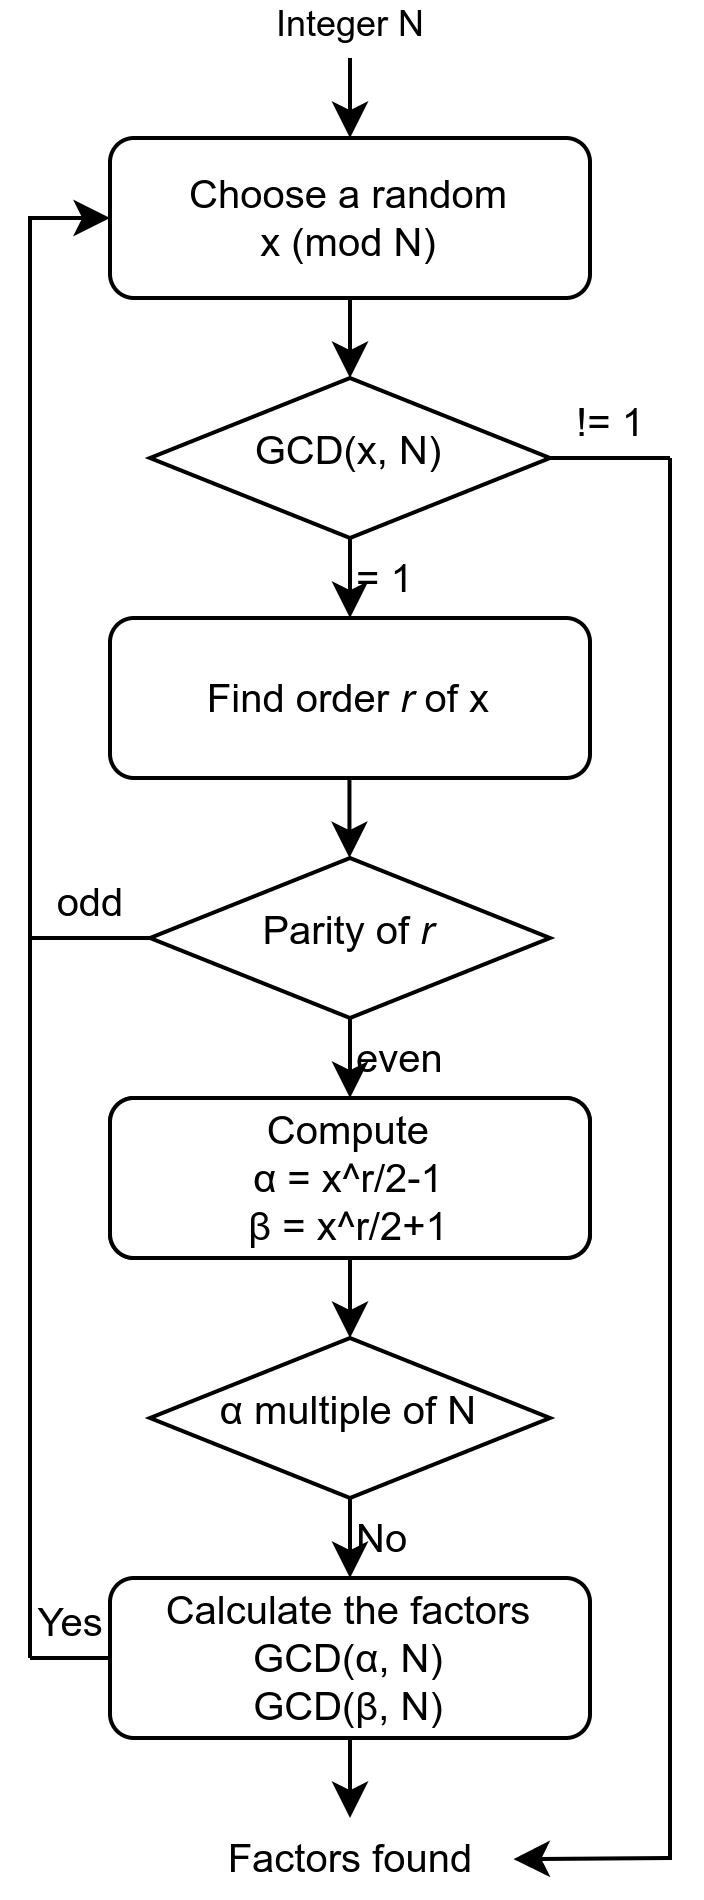
\includegraphics[width=0.4\textwidth]{shor}
    \caption{Shor's algorithm.}
    \label{fig:shor}
\end{figure}

The Greatest Common Divisor (GCD) of two integers is the largest positive integer that divides each integer. Finding GCD is an easy task also for classical computers, exploiting the Euclidean Algorithm \cite{knuth}.

The order \textit{r} is defined as the lowest integer that satisfies $x^r = 1 \pmod N$, and its finding is the bottleneck of classical computers. Shor, instead, showed that the problem could be solved in polynomial time by a quantum computer, drastically reducing the complexity of the overall factorization problem.

When a quantum computer capable of executing Shor's algorithm is available, the security assumptions of the DH algorithm will be compromised. Therefore, cryptographers devised a "quantum-resistant" algorithm for exchanging secret keys: Quantum Key Distribution.

\section{Quantum Key Distribution}
Quantum Key Distribution (QKD) refers to the generation of a secret key between two parties promising information-theoretical security, based on the fundamental laws of quantum mechanics: the algorithm's security does not depend on the computational power of the adversary. Therefore, these protocols can overcome the quantum computation's threat.

An essential and unique feature of QKD is the ability of the two communicating users to detect the presence of any third party aiming at gaining knowledge of the secret key. This capability is a consequence of a fundamental law of quantum mechanics: the process of measuring a quantum system disturbs the system itself. Therefore, a third party that wants to eavesdrop on the secret key must measure it somehow, thus introducing detectable anomalies. In the case of anomaly detection, the two parties abort the key generation process and agree on a new attempt.

The first and most-used QKD protocol is the one proposed by Charles H. Bennett and Gilles Brassard in 1984, known as BB84 \cite{bb84}. Here follows an introduction to the protocol, based on \cite{gagliano}.

\label{ch1:bb84}
In BB84, Alice and Bob are two entities sharing a quantum channel, usually an optical fiber where single-photon signals are transmitted, and an authenticated classical channel. Alice encodes the information on two different polarization bases: diagonal ($D = \{|\nearrow\rangle, |\nwarrow\rangle\}$) or rectilinear ($R = \{|\uparrow\rangle, |\rightarrow\rangle\}$). The protocol follows these steps:

\begin{enumerate}
    \item Alice chooses a random bit string $\beta$ and a random sequence $\pi$ of polarization bases
    \item Alice sends to Bob a train $\phi$ of photons encoded with a polarization state according to this table:
    \begin{table}[H]
    \centering 
        \begin{tabular}{| c | c | c |}
        \hline
        $\beta[i]$ & $\pi[i]$ & $\phi[i]$\\
        \hline \hline
        0 & D & $|\nearrow\rangle$\\\hline
        0 & R & $|\rightarrow\rangle$\\\hline
        1 & D & $|\nwarrow\rangle$\\\hline
        1 & R & $|\uparrow\rangle$\\\hline
        \end{tabular}
    \end{table}
    \item Bob chooses a random sequence $\rho$ of polarization bases
    \item Bob measures the polarization states of $\phi$ according to his choice $\rho$ and interprets the result \textit{r} as shown below:
    \begin{table}[H]
    \centering 
        \begin{tabular}{| c | c | c |}
        \hline
        $\rho[i]$ & $\phi[i]$ & $r[i]$\\
        \hline \hline
        D & $|\nearrow\rangle$ & 0\\\hline
        D & $|\nwarrow\rangle$ & 1\\\hline
        R & $|\rightarrow\rangle$ & 0\\\hline
        R & $|\uparrow\rangle$ & 1\\\hline
        \end{tabular}
    \end{table}
    \item Alice and Bob communicate their respective sequences of polarization bases through the authenticated classical channel.
    \item Both parties retrieve the \textit{sifted key}, discarding from $\beta$ and \textit{r} the bits measured by Bob with incorrect basis. The sifted key is composed only of bits encoded and detected with the same basis. Therefore, the number of correct bits cannot be determined a priori.
    \item Alice and Bob select a random sample of the sifted key to estimate the Quantum Bit Error Rate (QBER), which is the ratio between the number of wrong bits of the sifted key and the length of the sifted key. If the QBER is over an agreed threshold, the sifted key is considered insecure and discarded.
    \item Otherwise, Alice and Bob get the final secret key by applying classical post-processing algorithms to the sifted key, such as information reconciliation (for error correction) and privacy amplification \cite{privacyamp} (for the secretness of the key, guaranteeing that Eve cannot acquire any information about the key). The obtained key is the result of the QKD process.
\end{enumerate}

QKD relies on the fundamental properties of quantum mechanics. In contrast, DH key exchange and other classical protocols are based on the computational complexity of some mathematical problems.

Like all the other key exchange algorithms, QKD is only used to produce a secret key, not transmit any message data. Moreover, it does not offer authentication out of the box: it only focuses on the confidentiality of the secret key.

\label{ch1:length}
The secret key produced by a QKD algorithm is a sequence of bits whose length cannot be established a priori. Indeed, the sifted keys produced by Alice and Bob may differ in some positions due, for instance, to the non-ideality of the experimental realization or dark counts in the single-photon detection. These differences have to be discarded. Moreover, the length of the sifted key may be reduced by the classical post-processing algorithms mentioned above. Therefore, the bits generated by a quantum channel cannot be directly used as a key by encryption algorithms. In the next chapter, we will see how a Key Management Entity faces the problem of creating fixed-length keys exploiting bits produced with QKD.

\chapter{Key Management Entity}
\label{ch:kme}%
In the previous chapter, we summarized the history of the key exchange problem. Then, we pointed out Quantum Key Distribution as the solution to the problem. Following the fundamental laws of quantum mechanics, QKD can offer information-theoretic security. In this way, all the computational concerns that affect classical key-exchange algorithms such as Diffie-Hellman are avoided.

A secret sequence of bits produced by a couple of devices exploiting QKD cannot have a fixed length decided a priori, as explained in \ref{ch1:length}. However, the applications that want to exploit the secret key for encrypting a communication require the key to have a fixed length, usually a power of 2. For example, the Advanced Encryption Standard (AES) \cite{aes}, the most widely-used symmetric encryption algorithm, exploits keys of 128, 192, or 256 bits only.

Here we introduce the Key Management Entity (KME), the application managing the creation of fixed-length keys. We will see that this is not the only duty of the KME, and we will analyze all of them in detail.

Before diving into the KME, we formalize the concepts of Quantum Channel and Secure Application Entity. Hence, we focus on the distinction between sequences of bits produced by a Quantum Channel - which we call \textit{blocks} - and sequences of bits produced by the KME, denoted as \textit{keys}.

The following section analyzes the interaction between KME and the applications based on the standard ETSI GS QKD 014, described in detail. Then, the communication between KME and Quantum Channel is analyzed. In the end, the interaction between all the actors is explored in order to provide a complete overview of the system.

\section{Actors: KME, SAE and QC}
Here we introduce the leading entities of the quantum key distribution system we will describe.

First of all, a pair of devices able to build sequences of bits exploiting QKD protocols is called \textbf{Quantum Channel (QC)}. Each device is a QKD Entity (QKDE). The way a Quantum Channel produces sequences of bits has been described in the first chapter.

Each QKD Entity is linked to a \textbf{Key Management Entity (KME)}. The KME is the entity that manages keys in the network in cooperation with one or more other Key Management Entities.

Applications requesting one or more keys from a Key Management Entity are called \textbf{Secure Application Entities (SAE)}. In particular, the SAEs asking for the generation of new keys are called "master SAEs"; the ones asking for keys associated with given IDs are called "slave SAEs".

\section{Keys and blocks}
\label{kme:keys_vs_blocks}

We will distinguish "keys" and "blocks" from now on.

The product of a Quantum Channel is called \textbf{block}. A Universally Unique Identifier (UUID) \cite{uuid} identifies a block and contains a sequence of bits produced exploiting Quantum Key Distribution protocols: the \textit{block material}. Once again, it is essential to underline that the block material has a length that cannot be established a priori.

Instead, the product of a Key Management Entity will be called \textbf{key}. A UUID also identifies a key. It contains a sequence of bits, often referred to as \textit{key material}. However, the length of the key material can be determined by the KME. We will see that a key is built exploiting bits of one or more blocks.

The figure below quickly shows the leading entities of the network and what kind of information they exchange. QCs provide blocks to KMEs, while KMEs provide keys to SAEs.

\begin{figure}[H]
    \centering
    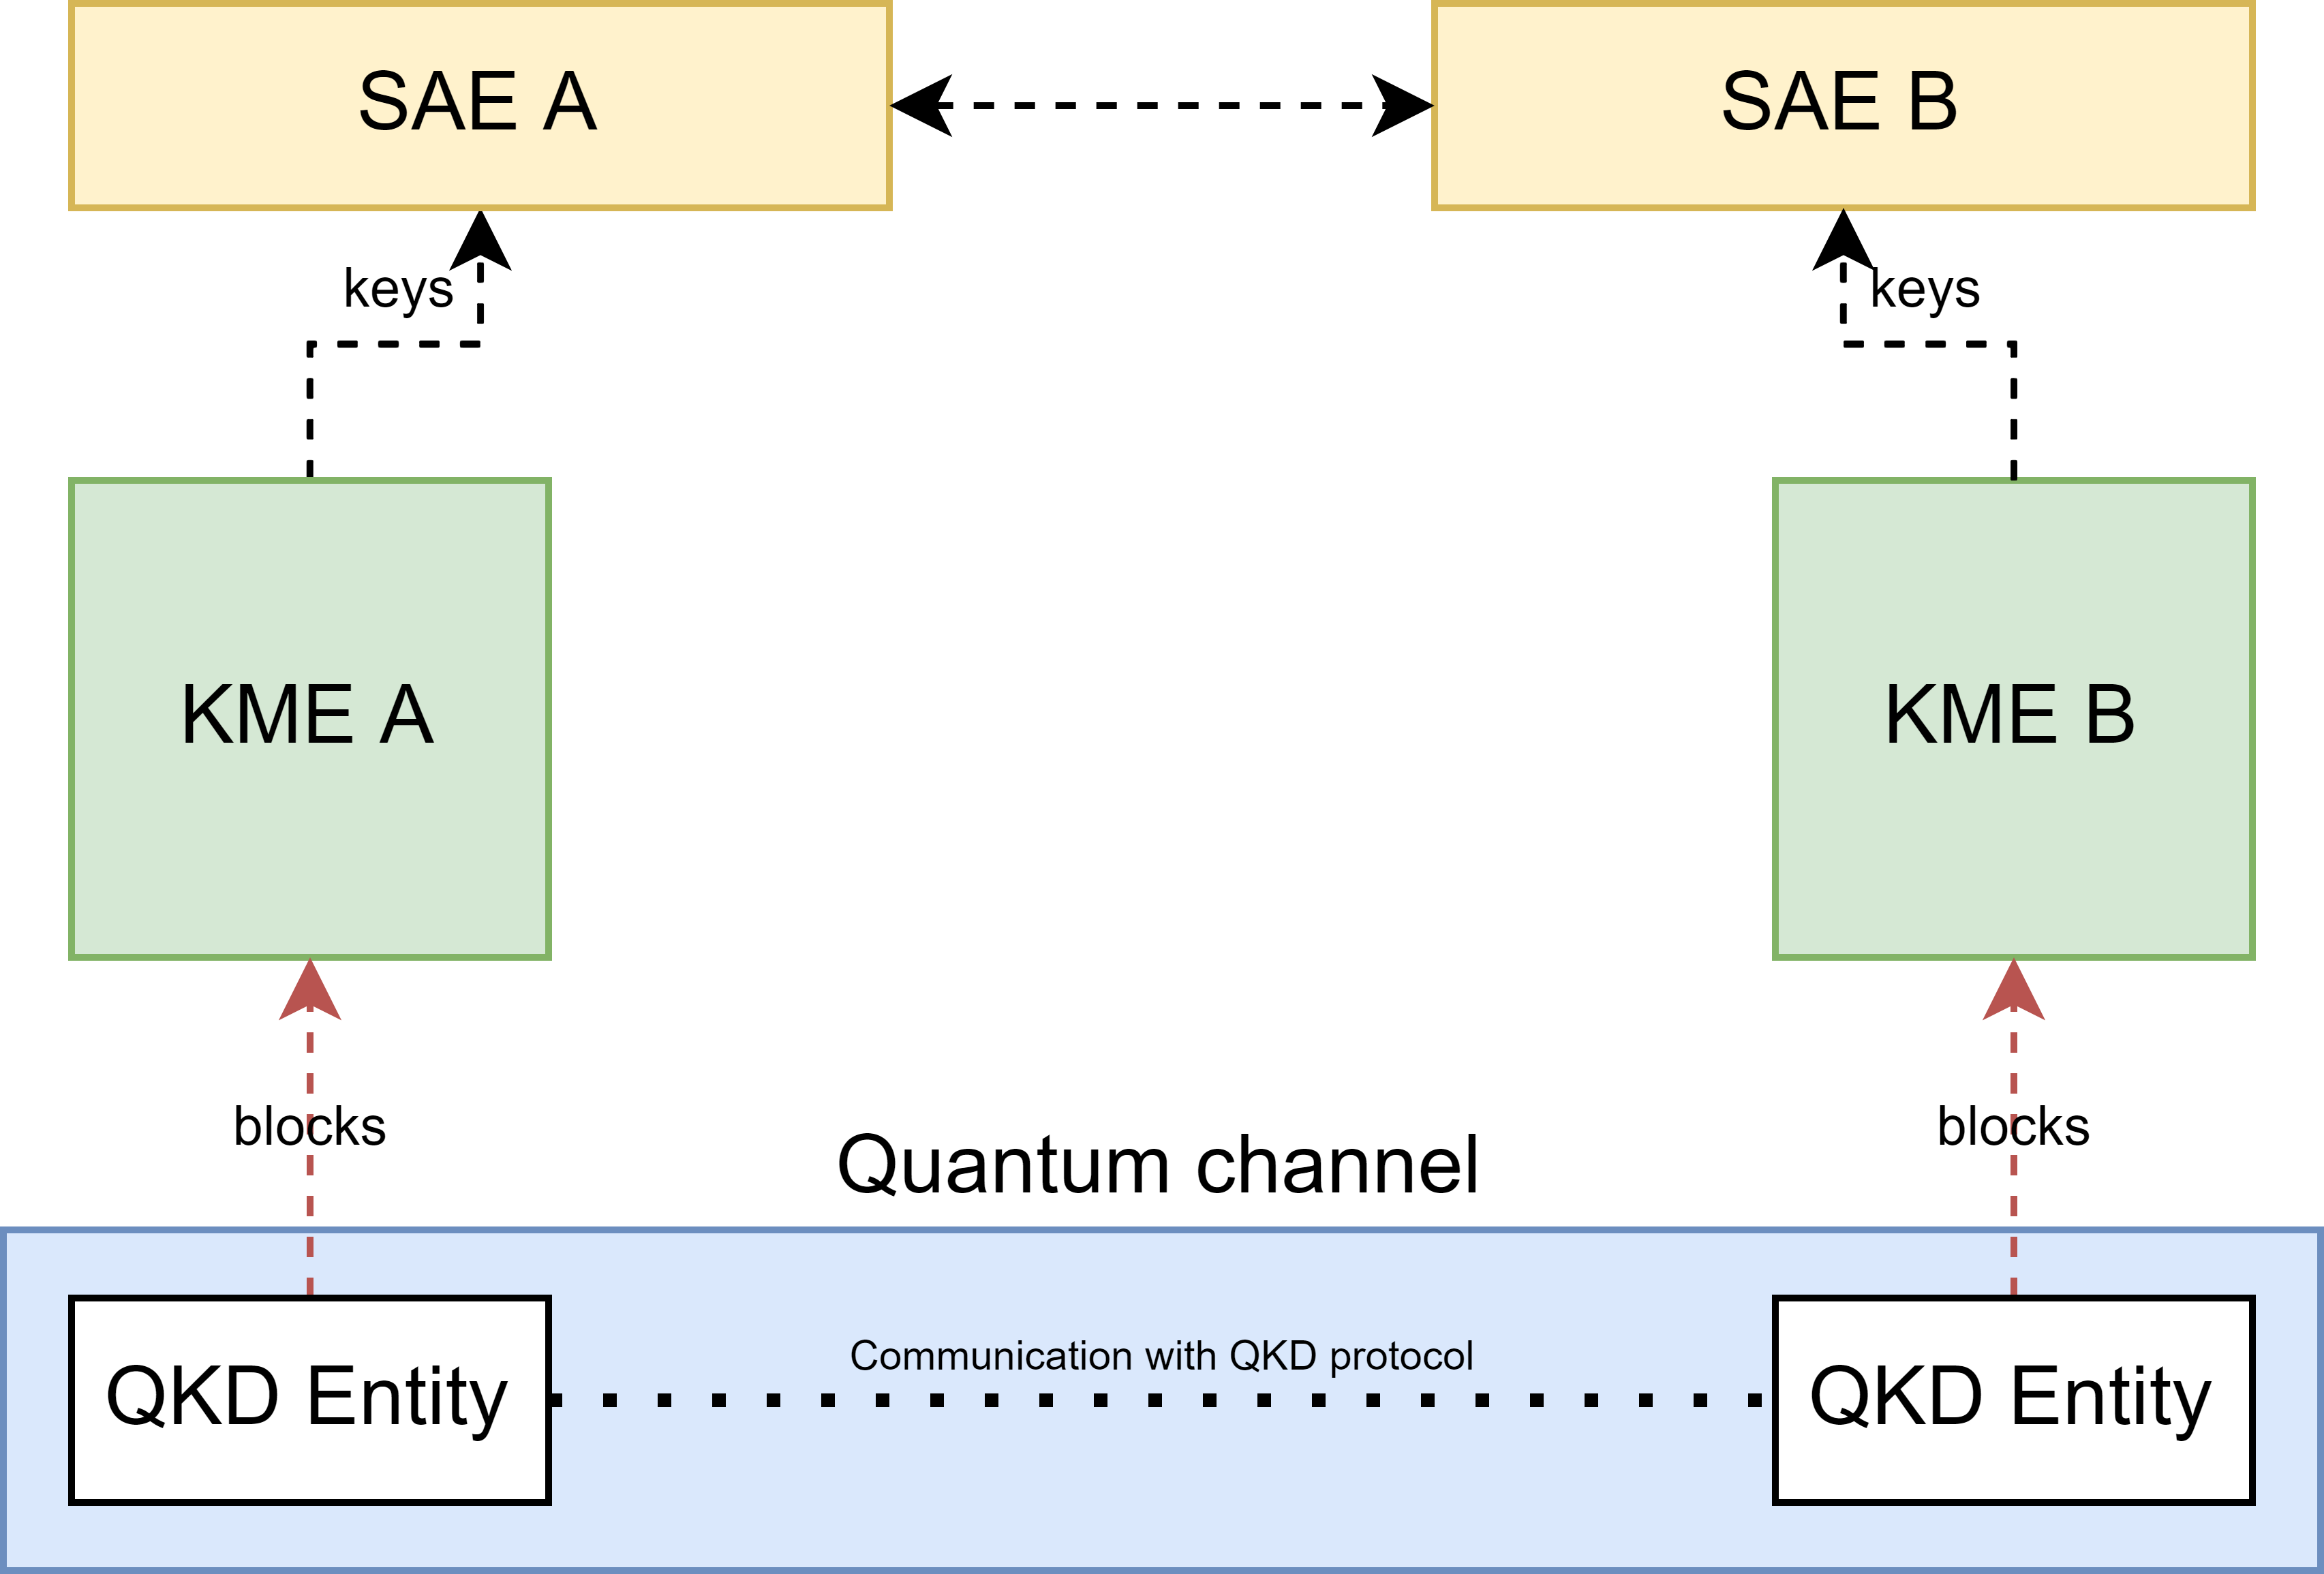
\includegraphics[width=0.8\textwidth]{overview}
    \caption{An overview of the network.}
    \label{fig:overview}
\end{figure}

\section{The interaction between the KME and the SAE}
This section will focus on the interaction between a Key Management Entity and one or more Secure Application Entities. The interface between these two entities has been implemented following standard ETSI GS QKD 014 \cite{etsi014}.

The standard ETSI GS QKD 014 defines an Application Programming Interface (API) that SAEs can exploit to send requests to KMEs. Each request is made through the HTTP protocol \cite{http}, the most widely-used protocol for internet communication. Data in the message body of HTTP requests from SAE to KME and HTTP responses from KME to SAE are encoded in JSON format \cite{json}.

In particular, an application may request:
\begin{itemize}
    \item the generation of one or more new keys
    \item the keys associated with one or more given key IDs
    \item the status of the KME (e.g., how many keys the KME can produce for each request, the maximum length of a produced key...)
\end{itemize}

There is an interface defined by the standard mentioned above for each of these three requests.

In the following sub-sections, we will dive into the specification of each interface.

\subsection{Generating keys}

\subsubsection{Key generation request}
\label{kme:key_gen}

A SAE that needs the generation of N keys of equal size S may use the HTTP GET method \textit{/enc\_keys}, specifying the "number" and the "size" as request parameters.

For example, if a SAE wants two keys of length 256, it may send an HTTP GET request with the following path:
\mint{latex}{/enc_keys?number=2&size=256}

There may be situations where the SAE wants to communicate some extra information to the KME. In this case, the SAE may exploit the HTTP POST method \textit{/enc\_keys}. Instead of specifying the "number" and "size" parameters, the HTTP POST method has a body whose data format is defined as a Key Request JSON data format. The Key Request JSON data format looks like this:

\usemintedstyle{borland}
\begin{minted}{json}
{
    "number": 2,
    "size": 256,
    "extension_mandatory": [
        { "abc_route_type": "direct" },
        { "abc_transfer_method": "qkd" }
    ],
    "extension_optional": [
        { "abc_max_age": 30000 }
    ]
}
\end{minted}

The "number" and "size" fields have the same meanings as the corresponding URL parameters.

"extension\_mandatory" is an array of name/value pairs representing extension parameters. The KME shall handle them or return an error.

"extension\_optional" is also an array of extensions specified as name/value pairs, but the KME may ignore these.

For more details on the Key Request JSON data format, see page 15 of the standard mentioned above.

\subsubsection{Key generation response}
\label{kme:key_container}
Despite the HTTP request received, the KME tries to generate the requested number of keys. How the KME produces keys will be discussed in the following sections. If the KME can produce the requested number of keys with the needed length and respect the mandatory extensions, its HTTP response will have a body containing a Key Container JSON data format. The following is an example of a Key Container JSON data format:

\begin{minted}{json}
{
  "keys": [
    {
      "key_ID": "ed4a8b14-0f5e-44c3-a28c-46e3df35dda4",
      "key": "jj86XIbUR9LVRVJaqoxcgw9mBaVzQHBtc8JEh9DUgAA="
    },
    {
      "key_ID": "23e0dfa1-e6f8-4477-a2c8-c7b0f9684769",
      "key": "aYXpqHpBgtH0rd7qubqTpSQ36fCReDeG6MBWPhkD/LI="
    }
  ]
}
\end{minted}

The Key Container is an array of keys. For each key, the UUID and the key material are given. Notice that the standard defines the key material field as "key". The key material is encoded as a base64 string \cite{base64}. Base64 is a binary-to-text encoding scheme designed to carry data stored in binary formats across channels that only reliably support text content.

For more details on the Key Container JSON data format, see pages 16-17 of the standard mentioned above.

Here is an example overview of a successful key generation request:
\begin{figure}[H]
    \centering
    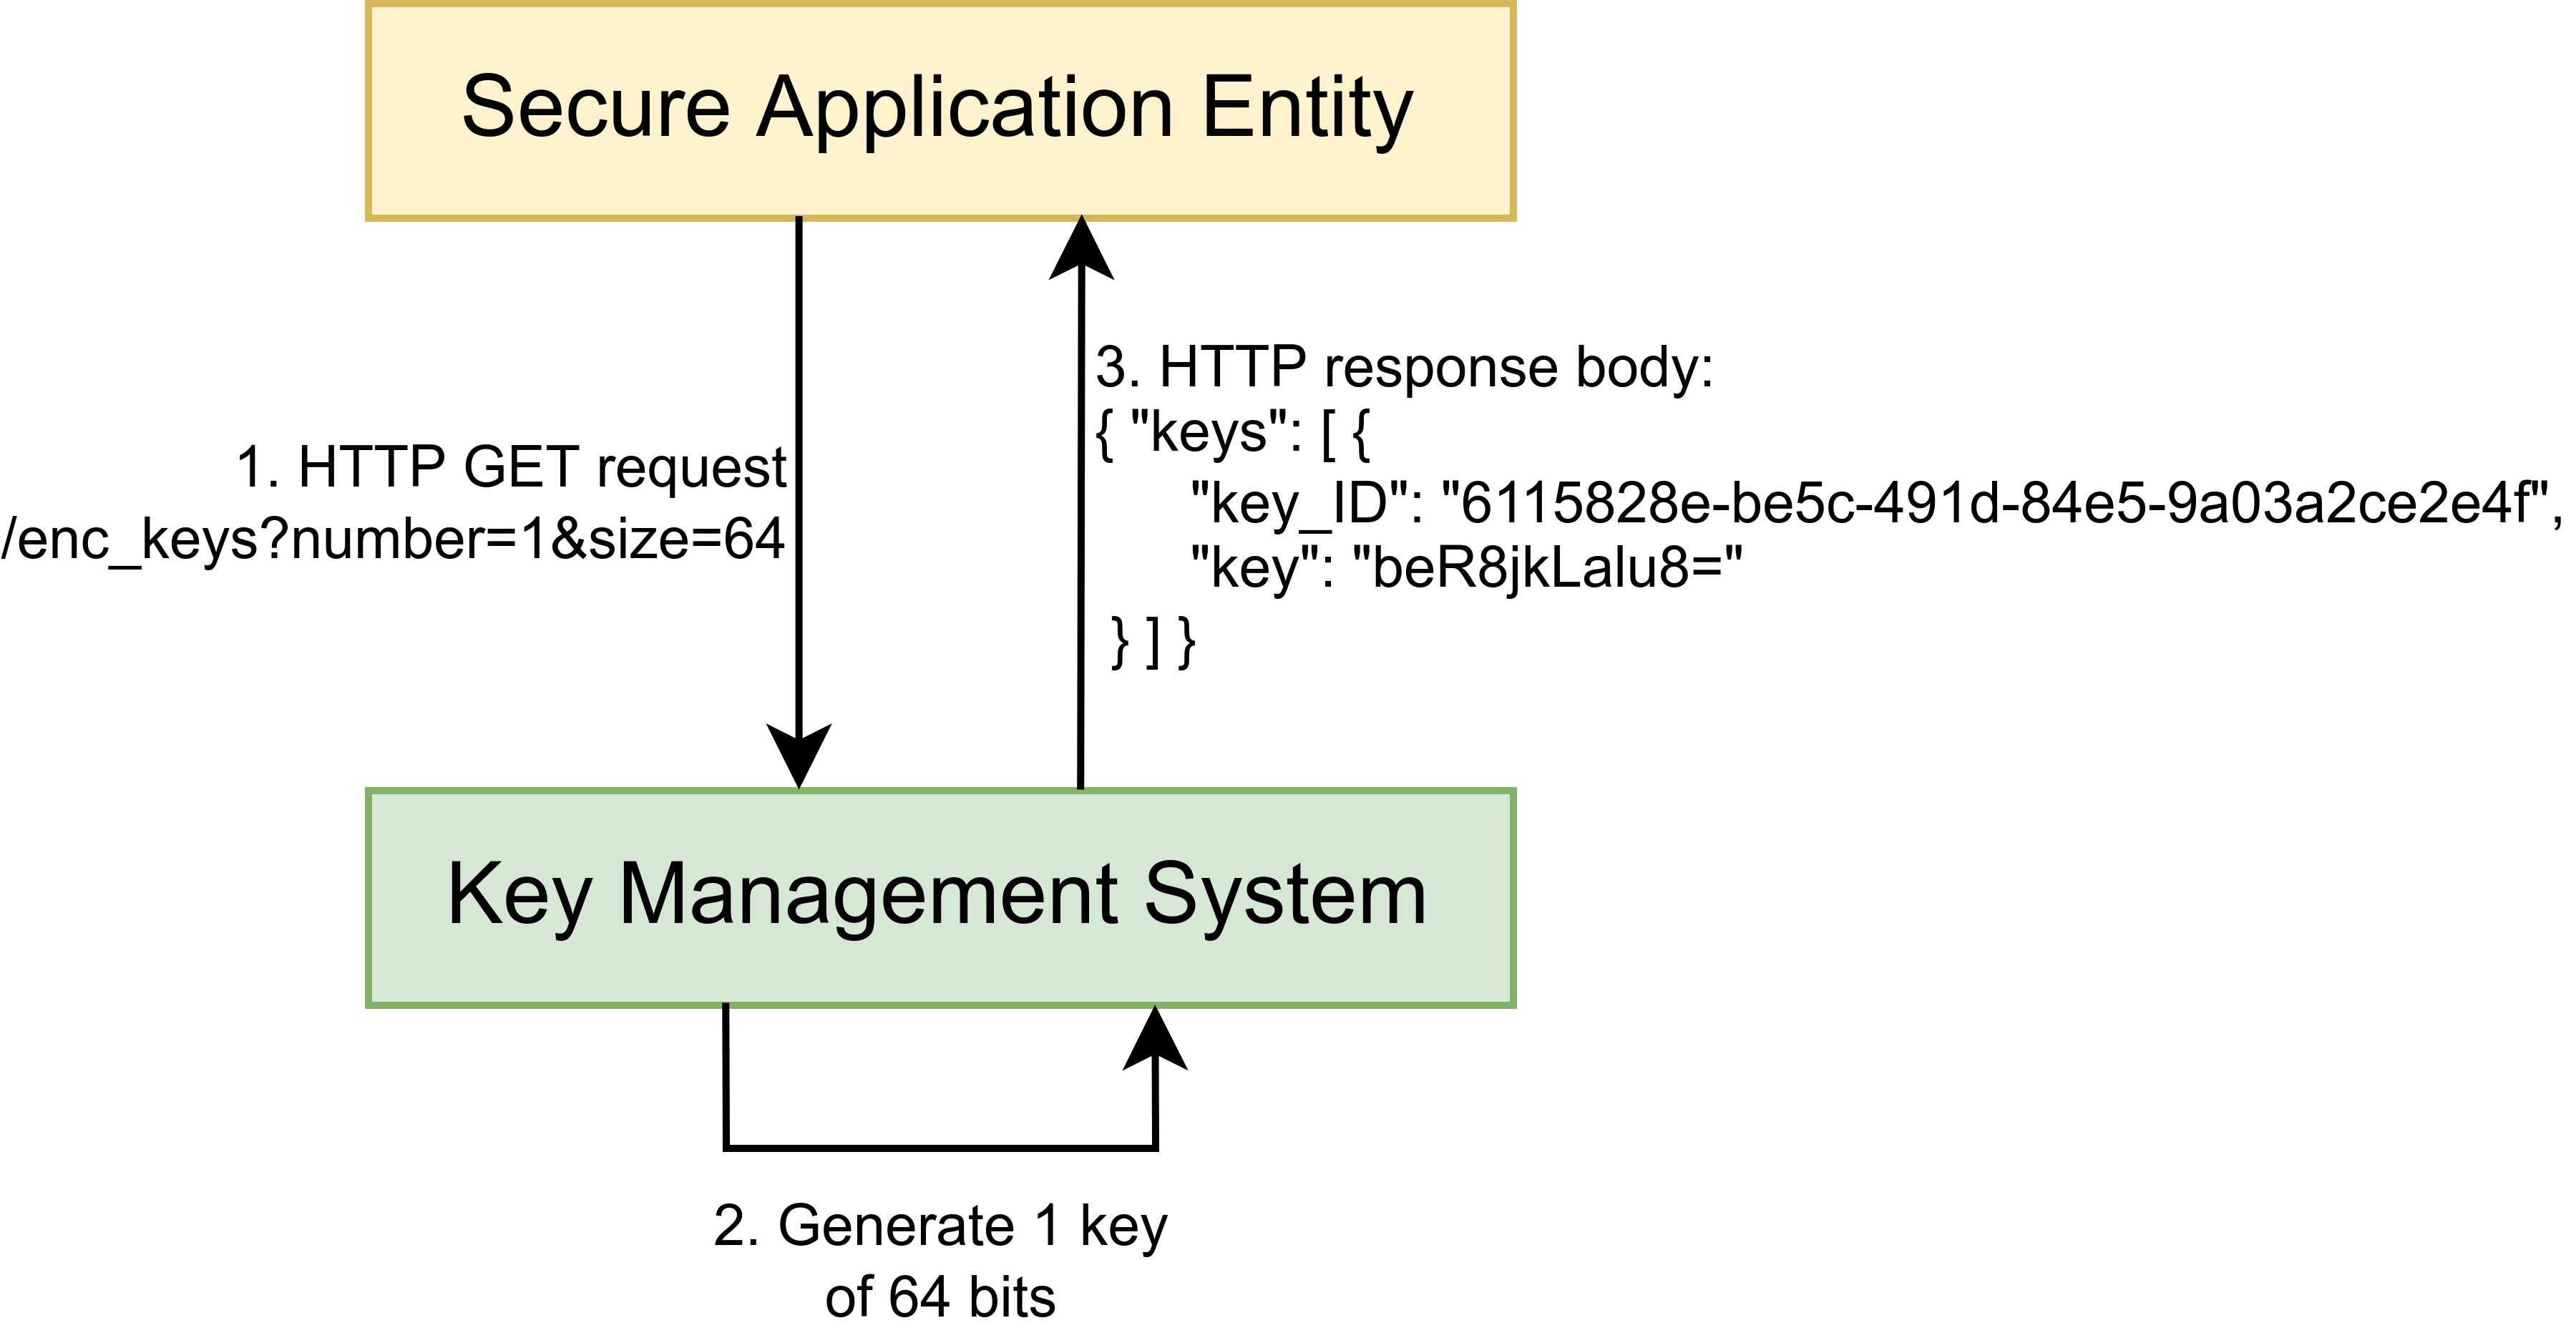
\includegraphics[width=0.8\textwidth]{Images/get_key.png}
    \caption{An example of a successful key generation request.}
    \label{fig:get_key}
\end{figure}

\subsection{Getting keys by ID}

\subsubsection{Keys by IDs request}
After one master SAE requests the generation of a new key, it communicates the UUID of that key to one or more slave SAEs. These can ask their KME to get the key material associated with a given key UUID.

A slave SAE that needs to retrieve the key associated with a given UUID can use the HTTP GET method \textit{/dec\_keys}, specifying the "key\_ID" as a request parameter.

For example, if a SAE wants to retrieve the key material associated to the key ID "ed4a8b14-0f5e-44c3-a28c-46e3df35dda4", it should send an HTTP GET request with the following path:
\mint{latex}{/dec_keys?key_ID=ed4a8b14-0f5e-44c3-a28c-46e3df35dda4}

Sometimes, one SAE may need to request the keys associated with multiple key IDs. In this case, the SAE may exploit the HTTP POST method \textit{/dec\_keys}. Instead of specifying the "key\_ID" parameter, the HTTP POST method has a body whose data format is defined as a Key IDs JSON data format. The Key IDs JSON data format looks like this:

\begin{minted}{json}
{
  "key_IDs": [
    { "key_ID": "ed4a8b14-0f5e-44c3-a28c-46e3df35dda4" },
    { "key_ID": "23e0dfa1-e6f8-4477-a2c8-c7b0f9684769" }
  ]
}
\end{minted}

\subsubsection{Keys by IDs response}
As shown in the figure above, a Key IDs JSON object is an array of key IDs. If the KME can retrieve the key of each key\_ID specified in the request body, the operation is considered successful. The HTTP response body will contain a Key Container JSON object with all the keys requested. More details about Key Containers are available in the previous section.

Otherwise, if one or more keys associated with the given UUIDs cannot be reconstructed, the HTTP response will report a failure. The HTTP protocol gives the response's status by the so-called "HTTP status code", an integer number of three digits. For example, a successful GET request has an HTTP status code of 200. A failure is usually reported with a status code starting with digit 4, such as "400". For more details about HTTP status codes, please see \cite{http_status_codes}.

The way the KME retrieves a key, given its UUID, is described in the following sections.

Here is an example overview of a successful key by ID request:

\begin{figure}[H]
    \centering
    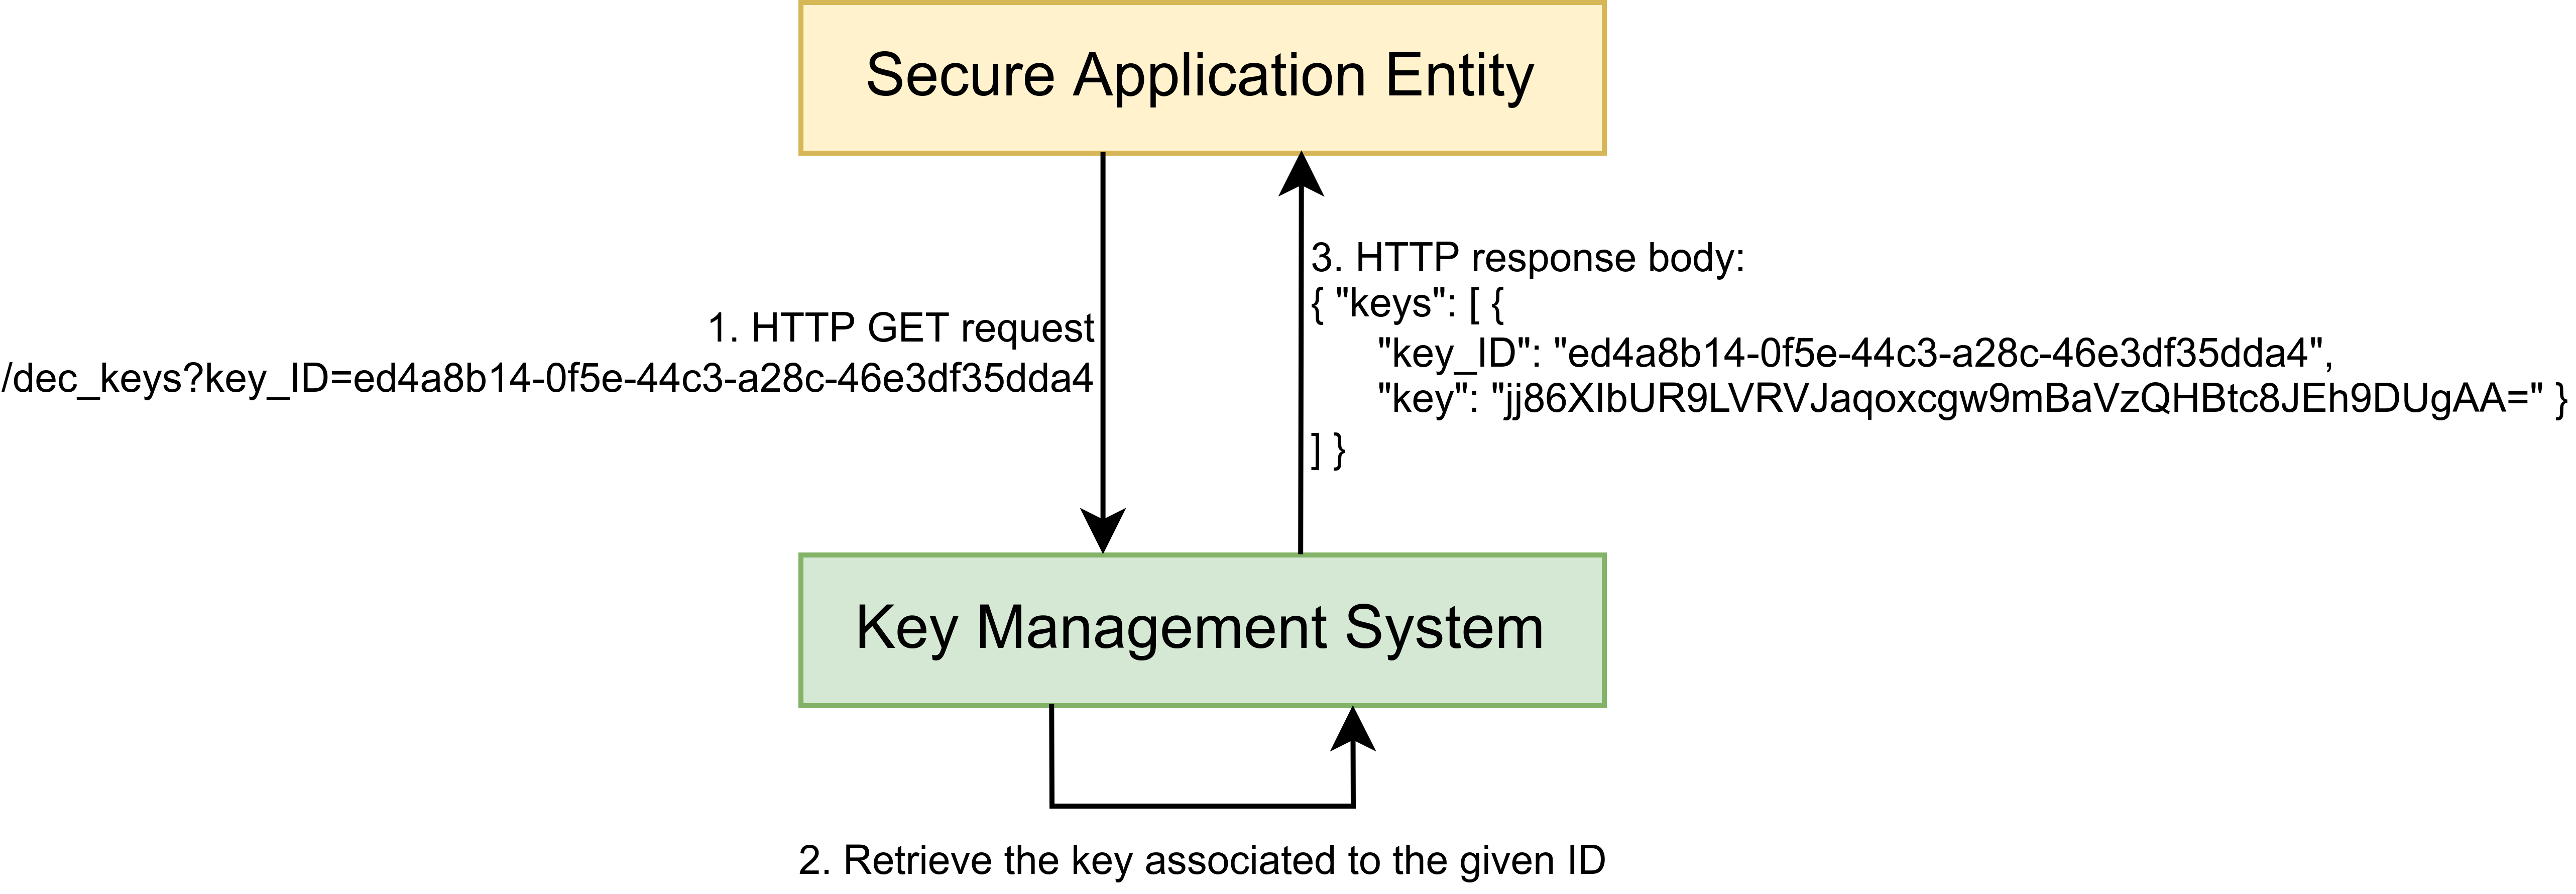
\includegraphics[width=1.0\textwidth]{Images/get_key_by_id.png}
    \caption{An example of a successful key by ID request.}
    \label{fig:get_key_by_id}
\end{figure}

\subsection{Requesting the status of the KME}
A Secure Application Entity may request the status of the Key Management Entity through the HTTP GET method available at path \textit{/status}.

When asked, the KME sends to SAE an HTTP response whose body contains a Status JSON object. The status JSON object includes some useful fields like:

\begin{itemize}
    \item key\_size: the default size, in bits, of key the KME can deliver to the SAE
    \item max\_key\_per\_request: the maximum number of keys a SAE may request with a single HTTP call
    \item max\_key\_size: the maximum size, in bits, of key the KME can deliver to the SAE
\end{itemize}

For a complete list of the fields inside a Status JSON object, please see page 14 of the standard mentioned above. 

\section{The interaction between the KME and the QC}
\label{kme:qc}

The previous section examined the interaction between KME and SAE, providing an overview of the standard ETSI GS QKD 014, exploited to implement the interface between the two entities mentioned above.

This section focuses on the interaction between the KME and a QKD Entity that is part of a Quantum Channel. For brevity, we often say: "The interaction between the KME and the Quantum Channel (QC)".

A Quantum Channel is a pair of devices that can securely exchange a secret sequence of bits, exploiting Quantum Key Distribution protocols. The product of a QKD exchange is called "block". Each block is identified by a UUID and contains the sequence of bits resulting from the key exchange. That sequence is called "block material".

The interface between the KME and the QC is not standardized. In particular, our implementation of this interface is based on conventions established in Politecnico di Milano.

When the Quantum Channel produces a new block, each QKD Entity of that channel sends the block to its KME. Therefore, the two KMEs involved will have a copy of the same block. In the following sections, we will see how a KME can produce keys starting from blocks and how it can communicate with the other KME to re-build that key.

Right now, we will specify how the QC sends blocks to KMEs.

The QKD Entity and the corresponding KME are linked through TCP socket connection \cite{socket}, a network-level API interface that allows two endpoints to communicate through a network. The API interface is simple: each KME is always listening on the socket connection, waiting for new blocks coming from the Quantum Channel.

When a QKD exchange is successful, each module of the Quantum Channel sends the very same block to the corresponding KME through the socket interface. In particular, the message is a JSON representation of the block. The Block JSON object has the following fields:

\begin{itemize}
    \item \textit{id}: the UUID of the block, chosen during the QKD exchange;
    \item \textit{key}: the block material, that is, the sequence of bits exchanged thanks to the QKD protocol. Notice that the block material is identified with the equivocal term "key" for compatibility reasons.
    \item \textit{time}: a timestamp identifying when the block has been produced;
    \item \textit{link\_id}: the UUID of the quantum channel that produced this block. Indeed, as it will be shown in \ref{ch4:exp3}, this implementation of the KME can receive and manage blocks coming from different quantum channels. The current chapter focuses on the interaction between the KME and only one Quantum Channel for clarity reasons.
\end{itemize}

When the KME receives a new block through the socket interface, it stores it locally. The block has to be stored confidentially not to break the security assumptions of the key management process. That block will then be used to build new keys or to re-build a key, given a key UUID.

\section{The internal functioning of the KME}
We analyzed how Secure Application Entities can request keys to Key Management Entities and how Quantum Channels can send blocks to KMEs. Now we are ready to dive into the internal functioning of the KME.

First, we will introduce two sub-sections of a KME devoted to storing blocks and instructions on how to re-build keys. Then, we will analyze the sequence of events that leads to the generation of a new key. In the end, we will focus on the process of retrieving keys, given their UUIDs.

\subsection{Local and shared storage}

\subsubsection{Storing blocks}
When the KME receives a newly-generated block from a Quantum Channel, it has to store it locally. This storage cannot be shared with anyone because it contains block material, the asset that has to be known only to the two collaborating KMEs.

In particular, a block stored in the local database contains the following pieces of information:

\begin{itemize}
    \item \textit{block\_id}: the UUID of the block;
    \item \textit{material}: the block material;
    \item \textit{timestamp}: the timestamp of the block;
    \item \textit{available\_bits}: an integer number that points out how many bits of the block were not exploited so far. When the block is inserted into the database, this field is equal to the length of the key material of the block. If, for example, the first ten bits of key material are exploited in order to build a key, the value of \textit{available\_bits} will be decreased by 10;
    \item \textit{link\_id}: the UUID of the quantum channel that produced this block.
\end{itemize}

Notice that, despite some changes in the name of the fields, \textit{available\_bits} is the only one added to the block by the KME when it has to store the block locally.

We will often refer to this local database as \textbf{local block DB}.

\subsubsection{Storing key instructions}
When the KME produces a new key, it has to store the instructions about how the key was built (i.e., which bits of which blocks were used to build the key material) in a database shared with the companion KME. The other KME will have to read those instructions to re-build the key. One KME cannot communicate the key material directly to the other KME: this would compromise the security assumptions of all the systems. The only communication of confidential bits between entities of the same kind is performed by the QKD Entities of the Quantum Channel, exploiting Quantum Key Distribution protocols.

The KME, after having created a key successfully, stores the instructions in the shared database. For each key, these pieces of information are stored:

\begin{itemize}
    \item \textit{key\_id}: the UUID of the key;
    \item \textit{instructions}: a list of instructions. Each instruction has the following structure:
    \begin{itemize}
        \item \textit{block\_id}: the UUID of the exploited block;
        \item \textit{start}: the index of the first bit of this block used in order to build the key material. Indexes start from 0 up to the length of the block material.
        \item \textit{end}: the index of the first bit of this block \textit{not} used in order to build the key material. It has to be a value greater than "start" and smaller or equal to the length of the block material. It is equal to the length of the block material only if the block material has been completely consumed.
    \end{itemize}
\end{itemize}

In our implementation of a KME, much care is taken to avoid repeated usage of the same bit to create two distinct keys.

The precise way instructions are created is described in the next section.

We will often refer to the shared database we have just described as \textbf{shared key DB}, or "shared DB".

\subsection{Generating new keys}
A master Secure Application Entity may request to the Key Management Entity the generation of new keys through the key delivery API implemented following the standard ETSI GS QKD 014, as seen in \ref{kme:key_gen}.

Now, we will describe how the KME manages the generation of N keys of size S.

The following procedure is repeated for each of the N keys requested:

\begin{enumerate}
    \item First, a new UUID is generated: it will be associated with the key after its material has been created.
    \item Then, construction of the key material begins. First, the KME picks up a block fragment from the local block DB. Then, it takes bits from the block material up to reaching the requested key length or up to finishing the bits of that block. Finally, the instruction pointing out the part of block material exploited is added to the list of instructions for that key.
    \item If the bits of the block material are exhausted and the requested key length is not reached, then the KME picks up another block from the local block DB and repeats the above process. 
    \item If the requested key length is reached, the KME stores the instructions for building that key in the shared database and proceeds to create the following key. Suppose the requested key length is reached, but the currently-exploited block has bits remaining. In that case, the block is re-inserted into the local block DB, coherently updating the value of its field \textit{available\_bits}.
    \item If all the N requested keys are generated, the KME returns them to the calling SAE through an HTTP response with status code 200, whose body is a Key Container that includes such keys. For more details about the structure of a Key Container, see \ref{kme:key_container}.
    \item If the KME does not find any available block fragment or in case of any other possible error, an HTTP response with status code 400 is returned. For more details about the status codes returned by the KME in case of errors, please refer to the standard ETSI GS QKD 014.
\end{enumerate}

The following figure shows the sequence of events that starts with a key generation request by a SAE and ends with the HTTP response given by the KME, containing the requested number of keys.

\begin{figure}[H]
    \centering
    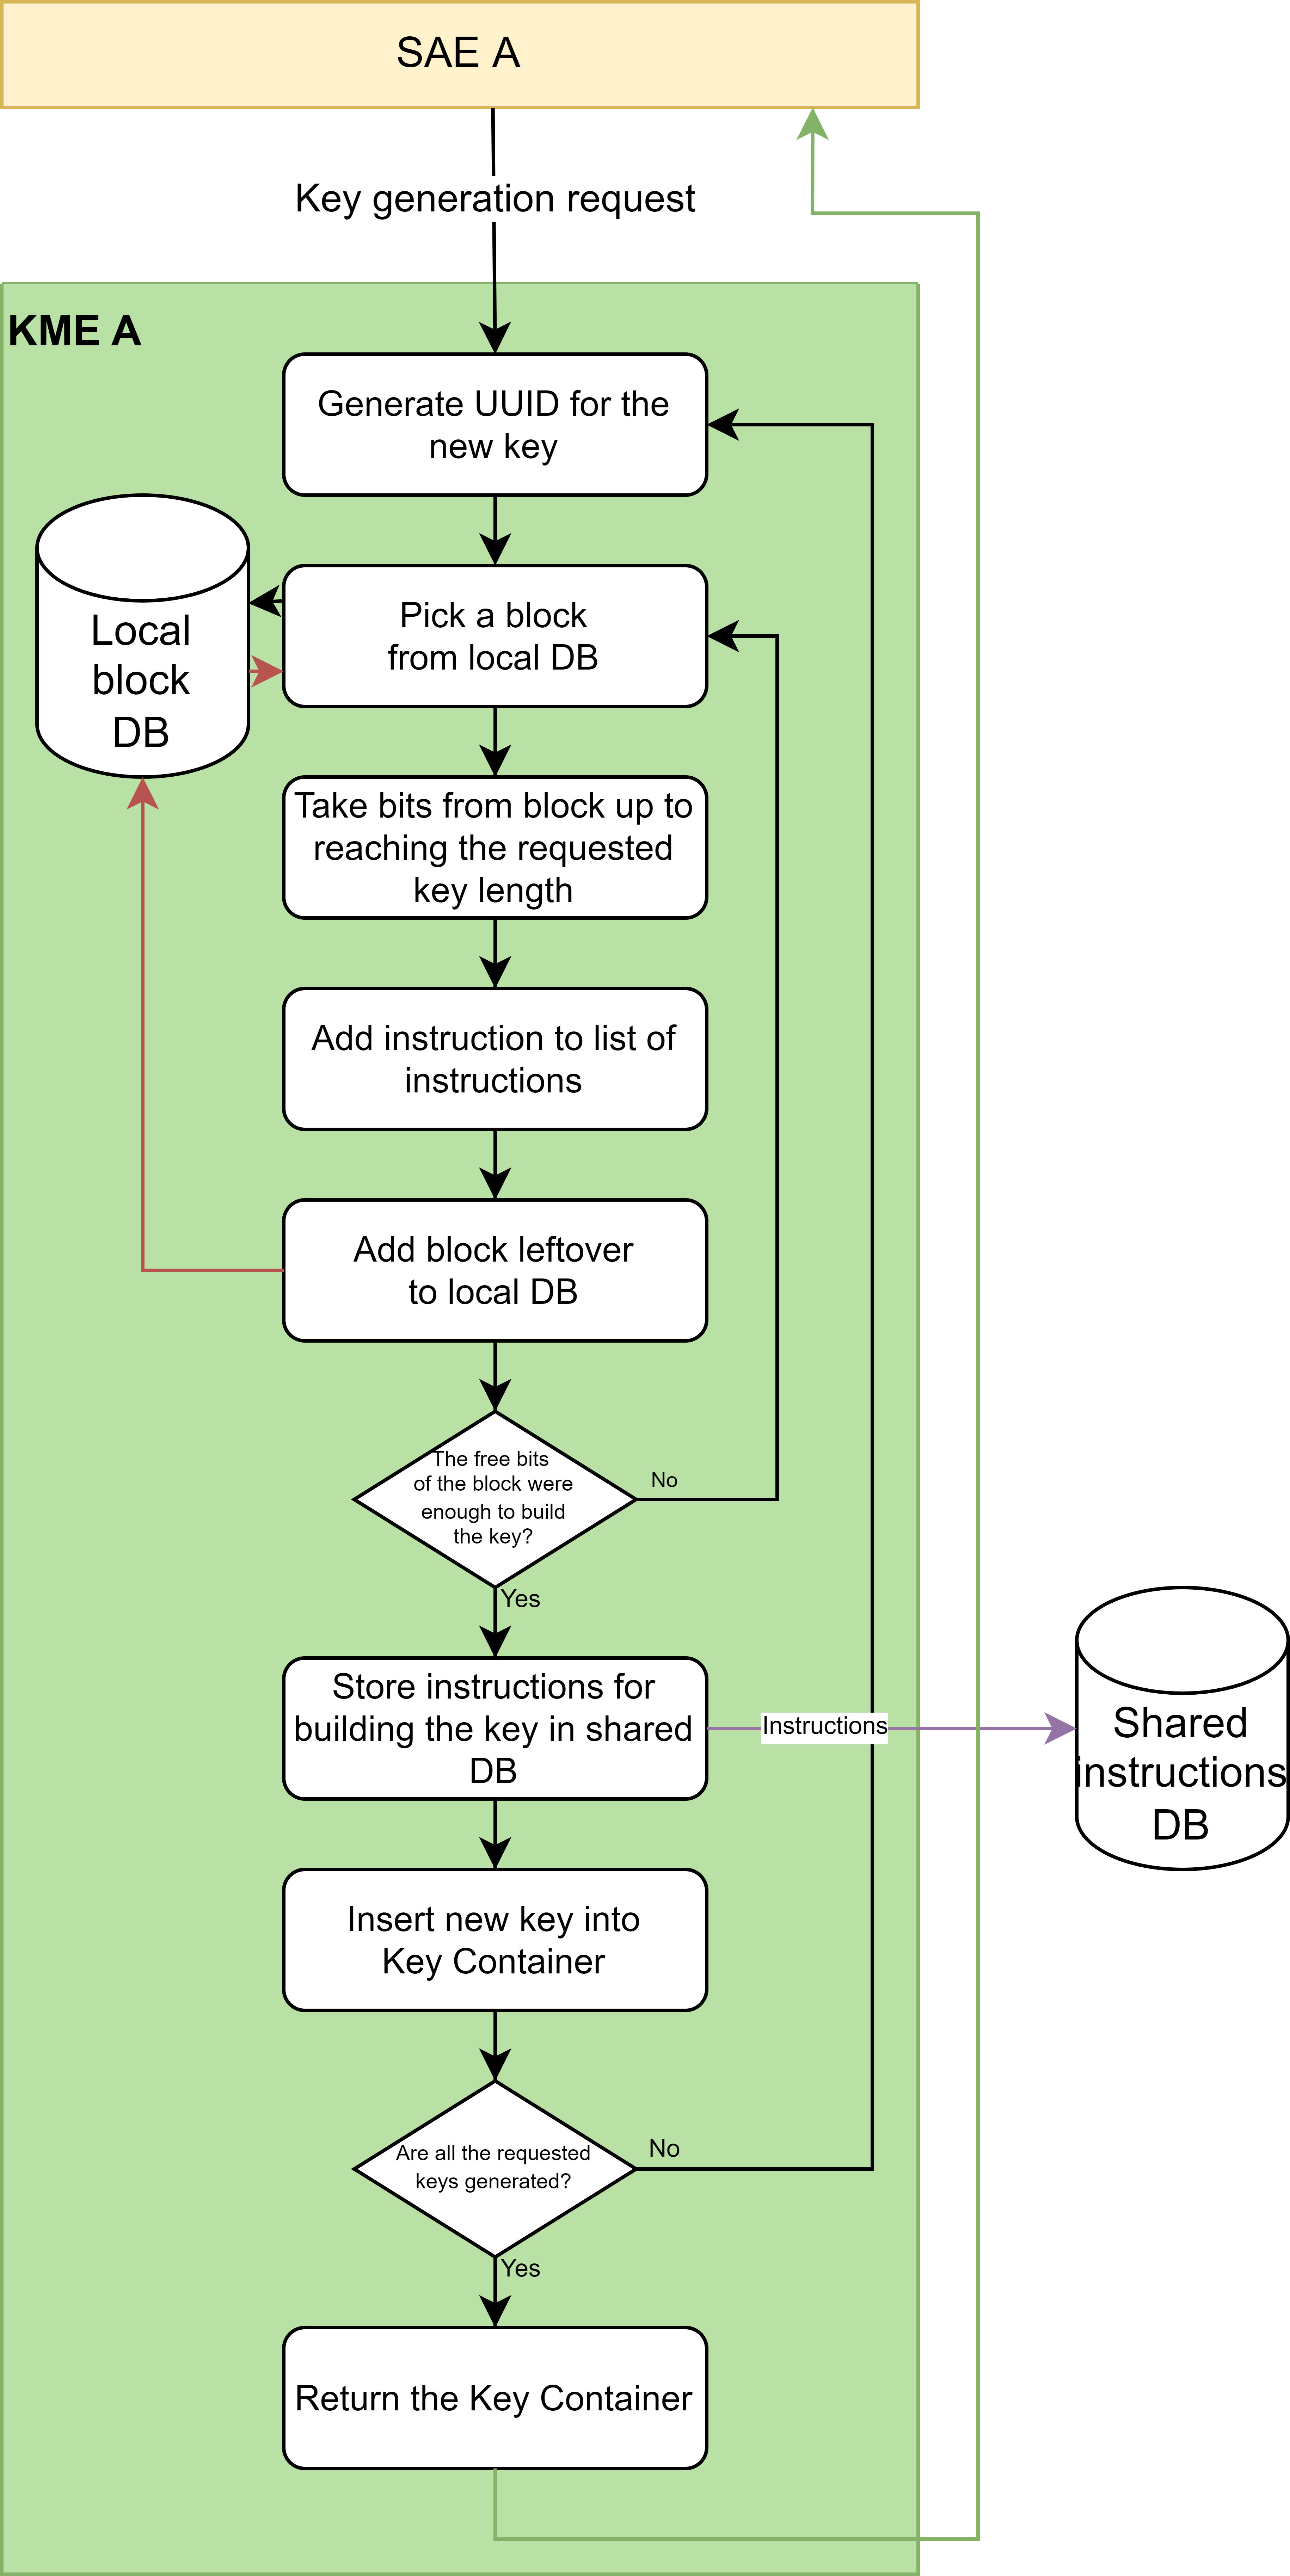
\includegraphics{Images/key_generation.png}
    \caption{The management of a key generation request.}
    \label{fig:key_generation}
\end{figure}

\subsection{Getting blocks by ID}
After one master SAE requested the generation of N keys of length S to one KME, other slave SAEs may request to retrieve those keys to the other KME. In this paragraph, we describe the process of retrieving keys, given their UUIDs, step by step.

When KME receives a request for getting keys associated with given UUIDs, for each UUID:

\begin{enumerate}
    \item First, it reads from the shared DB the instructions associated with the given UUID. If no instructions are associated with the UUID, the KME returns an HTTP response with status code 404.
    \item If there are instructions associated with the given key UUID, then the KME reads them. Each instruction contains the UUID of a block. Then, the KME retrieves that block from the local DB. Again, suppose there is no block associated with the given UUID. In that case, the KME returns an HTTP response with a failure status code.
    \item For each block retrieved, the KME extracts the bits pointed out in the corresponding instruction. This process allows to re-build the key material of the key with the given UUID.
    \item If a key is correctly re-built, it is inserted into the Key Container that will be the body of the HTTP response.
    \item If all the requested keys have been correctly re-built, the KME returns an HTTP response with status code 200, whose body is the Key Container that includes the keys re-built starting from their UUIDs.
\end{enumerate}

The following figure shows the sequence of events that starts with a key retrieval request by a SAE and ends with the HTTP response given by the KME, containing the requested keys. For simplicity and readability, it shows the path followed in case of a successful request.

\begin{figure}[H]
    \centering
    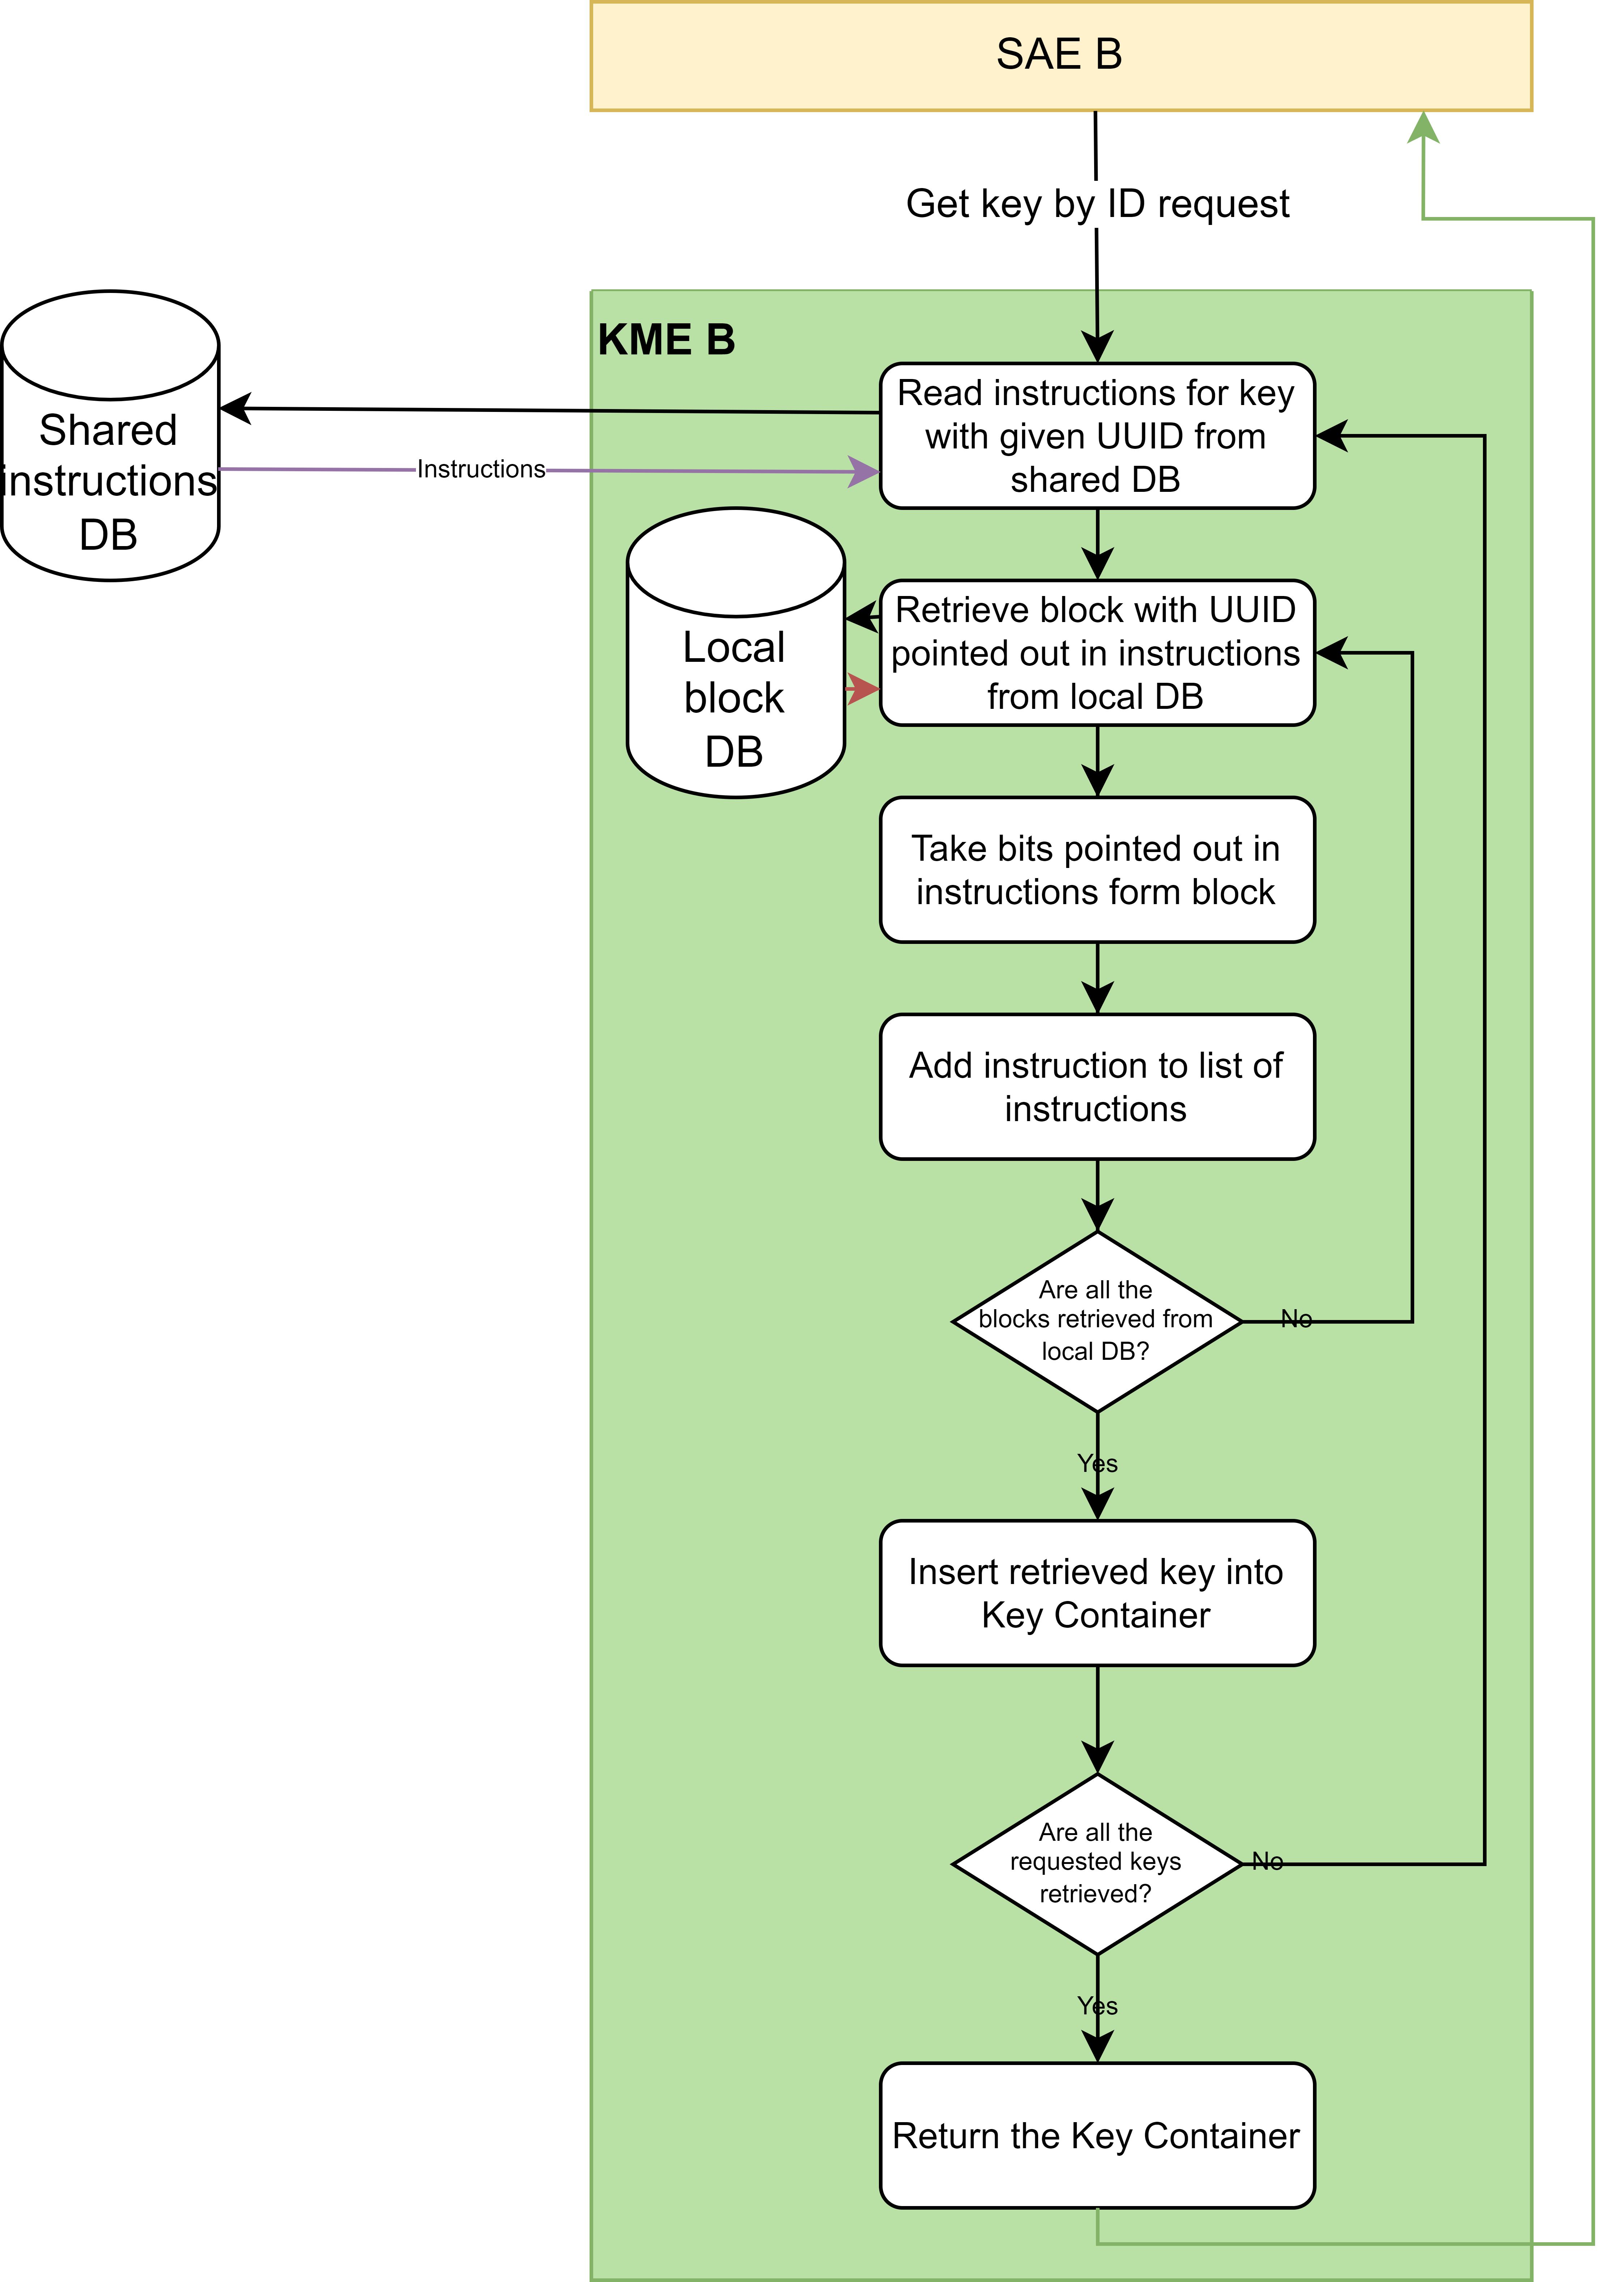
\includegraphics{Images/key_retrieval.png}
    \caption{The management of a key retrieval request.}
    \label{fig:key_retrieval}
\end{figure}

\subsection{The cooperation between KMEs}
At the end of this chapter, we can have a complete overview of the key management process.
It all starts with the request to generate one or more keys by a Master SAE to its KME through the API described in the ETSI standard. We refer to the Master SAE as "SAE A" and its KME as "KME A".
SAE A communicates the UUIDs of the keys received from KME A to other SAEs. We refer to them as "SAE B". SAE B is a Slave SAE, which requests from its KME - "KME B" - the keys associated with the UUIDs received from SAE A.
Finally, thanks to this process, the SAEs have the same keys, which have been generated and distributed confidentially, to be used, for example, for encrypting future communications.

The following figure summarizes the entire process of key distribution made possible thanks to Key Management Entities. We used the ID "abc" for the requested key for simplicity and readability. However, keep in mind that a UUID identifies the keys.

\begin{figure}[H]
    \centering
    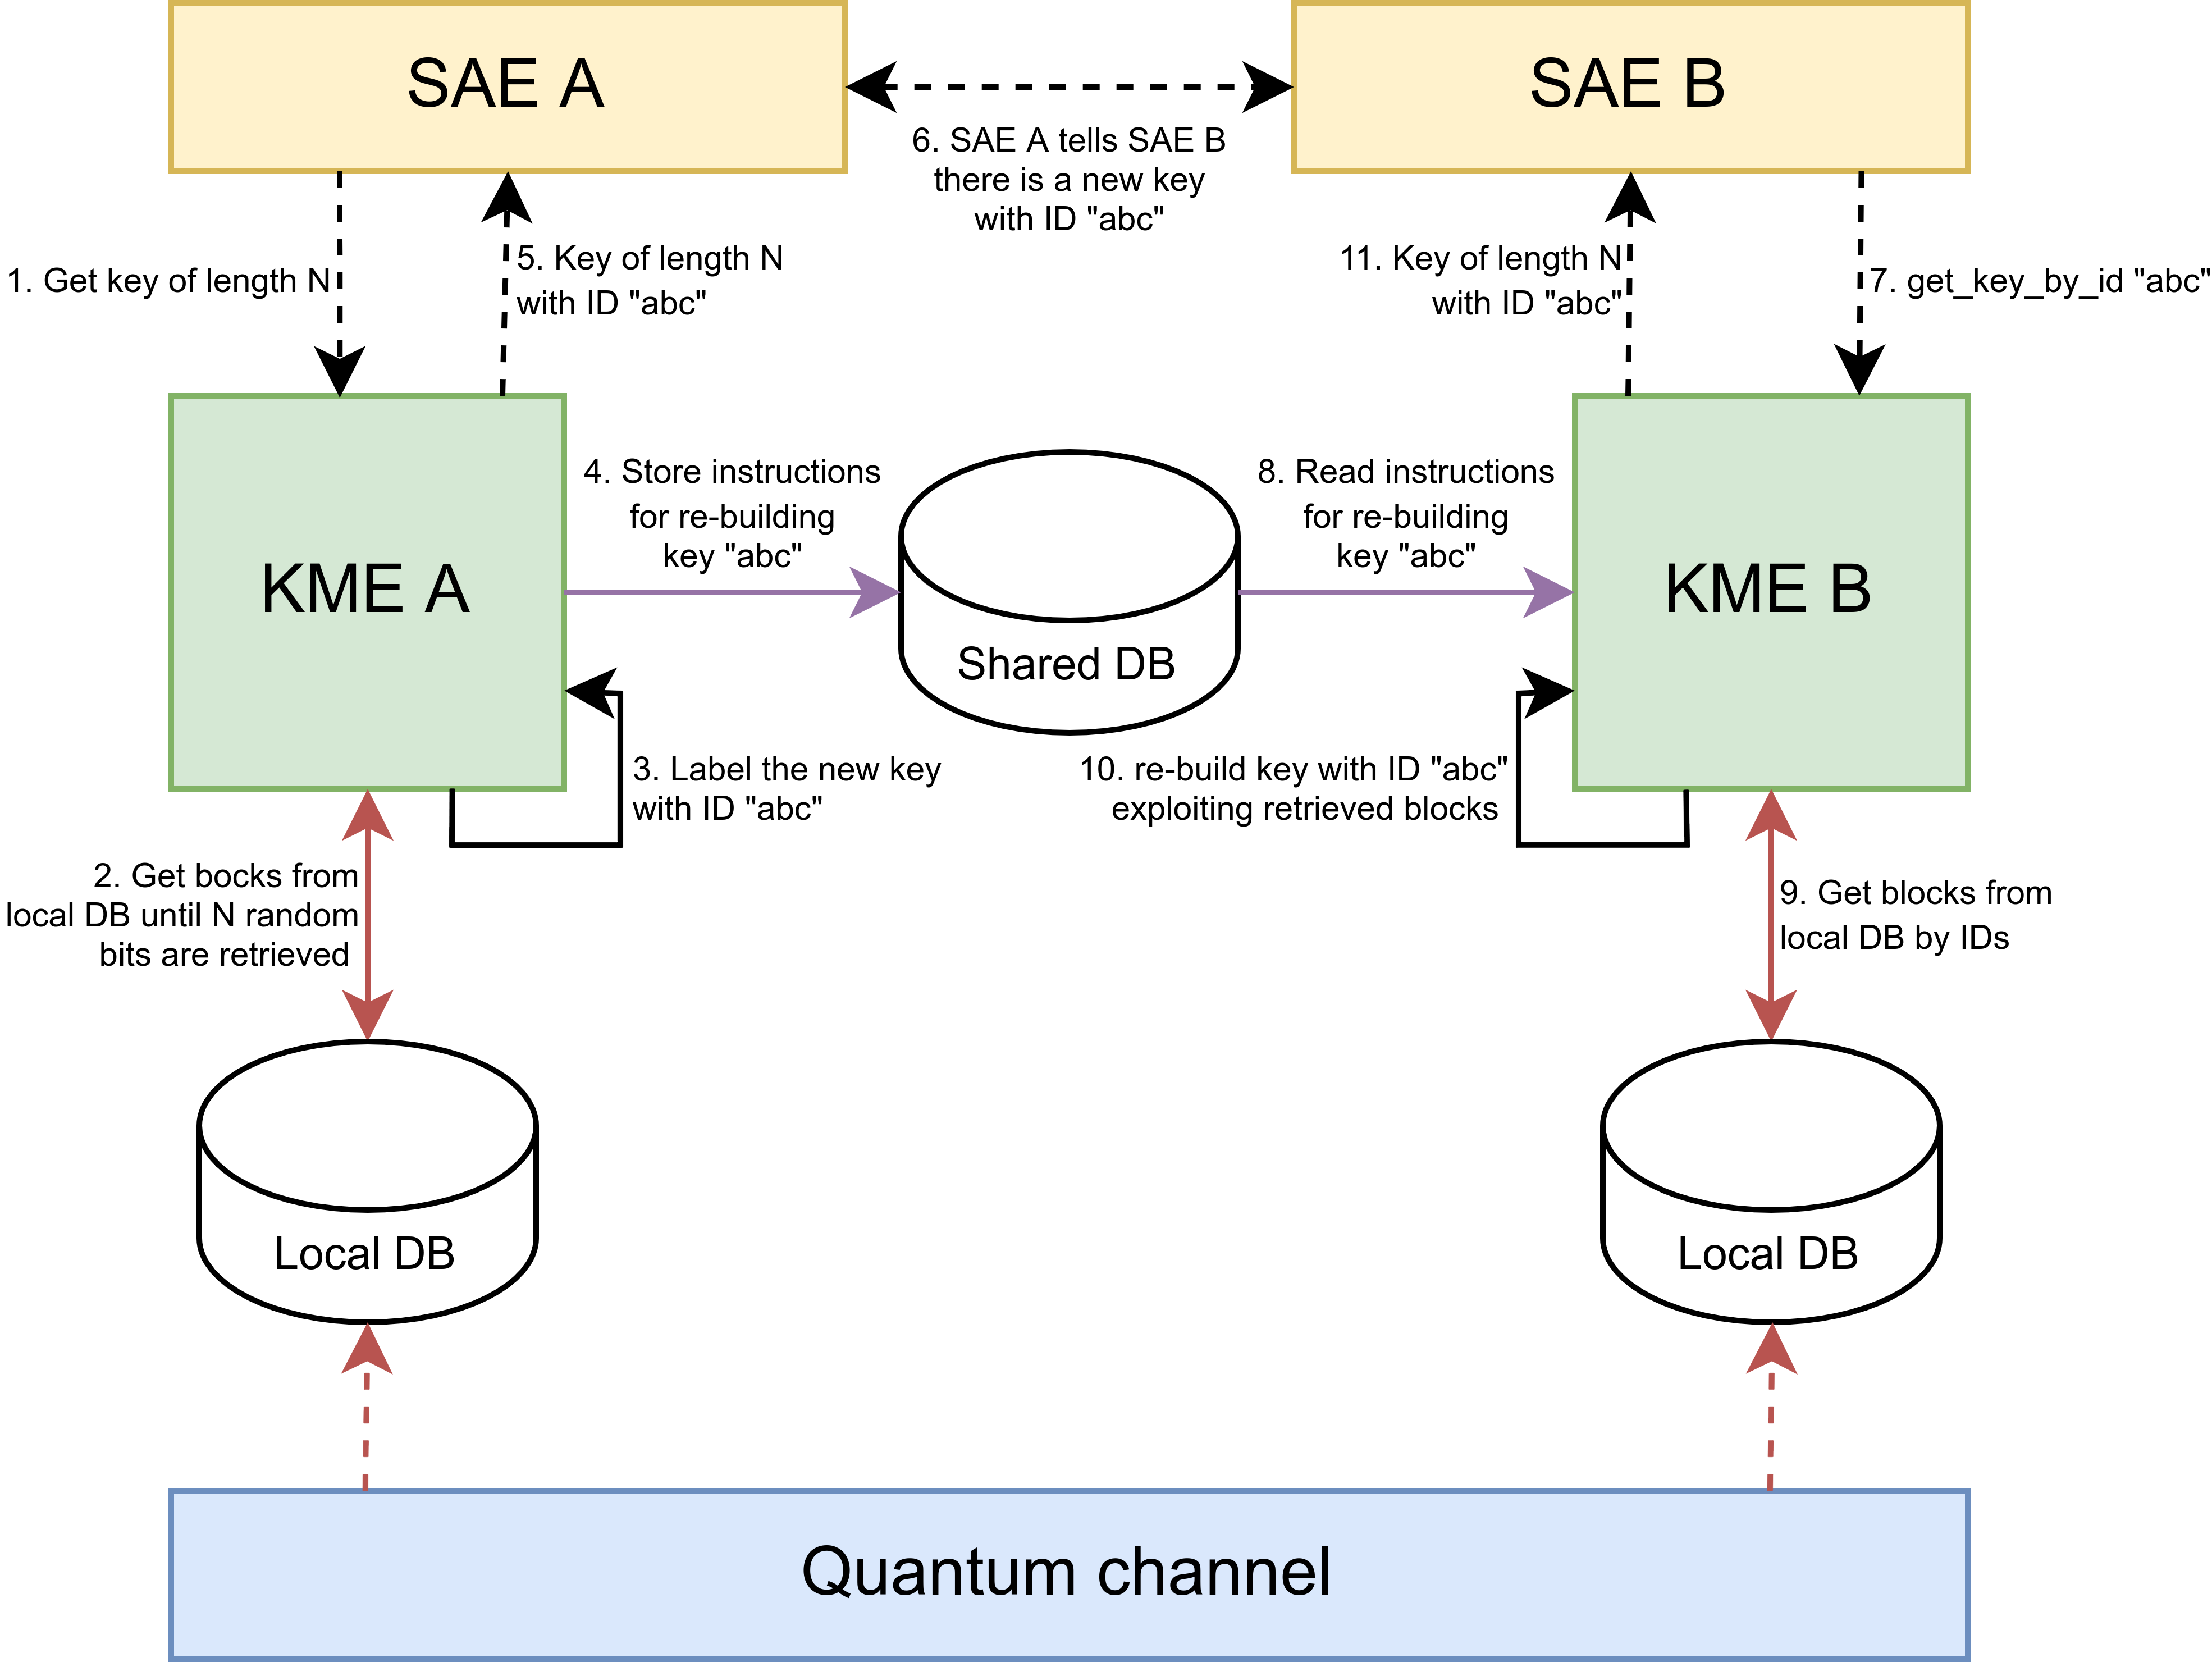
\includegraphics[width=1.0\textwidth]{Images/sequence_diagram.png}
    \caption{A complete overview of the key management process.}
    \label{fig:sequence_diagram}
\end{figure}

\chapter{Implementation of a Key Management Entity}
\label{ch:implementation}%

The previous chapter introduced the Key Management Entity (KME). Then, we described its interaction with Secure Application Entities (SAEs) and Quantum Channels (QCs). Next, we focused on the internal functioning of the KME, finally giving a complete overview of the key management process.

This chapter will focus on our implementation of a Key Management Entity.

The KME is implemented using Python \cite{python}, one of the most popular high-level programming languages nowadays. In particular, this implementation works only with a version of Python at least equal to 3.10, the most recent version at the time of writing.

In the following sections, we will introduce Poetry, the dependency management system of this project. Then, we will describe the software dependencies required to make this KME implementation work. After that, we will explain how to start one KME or a couple of cooperating KMEs. Next, we will describe the different modes of operation of the KME: development, testing, and production. In the end, we will focus on how the project has been tested.

\section{Software dependencies}

Within a software project, recurring problems are encountered. The solutions to these problems are pieces of software that developers reuse in multiple projects, at the cost of not having complete control over their development. They are called "dependencies".

The dependency management of this project is entrusted to Poetry. Poetry reads the project dependencies from a file called \textit{pyproject.toml}, and it allows to install all of them with a single command:

\begin{minted}{bash}
poetry install
\end{minted}

The dependencies can be distinguished into two groups: project and development dependencies. The former is necessary for making the KME work, and the latter is only required for development purposes. It is possible to avoid the installation of development dependencies using the following command instead of the above one:

\begin{minted}{bash}
poetry install --no-dev
\end{minted}

\section{How to start one KME}
In order to execute the program, Python 3.10 or higher must be installed on the operating system in use. Then, the following commands have to be executed in a terminal:

\begin{minted}{bash}
poetry install
poetry run python -m kme
\end{minted}

As discussed in the previous section, the first command forces Poetry to install all the project dependencies. The second command starts a Key Management Entity.

\begin{figure}[H]
    \centering
    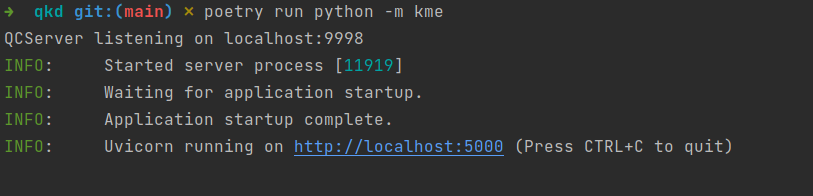
\includegraphics[width=0.9\textwidth]{Images/kme_start.png}
    \caption{A Key Management Entity started in a Linux terminal.}
    \label{fig:kme_start}
\end{figure}

\section{The web API interface}
\label{kme:api}

Thanks to FastAPI, one of the project's dependencies, the KME makes an API interface available as a web page by default. The KME displays the URL link to this interface in the terminal just after starting. The following figure shows an overview of the web page: it shows all the SAE's methods to interact with the KME. The web API interface can simulate the execution of an HTTP request to the KME.

\begin{figure}[H]
    \centering
    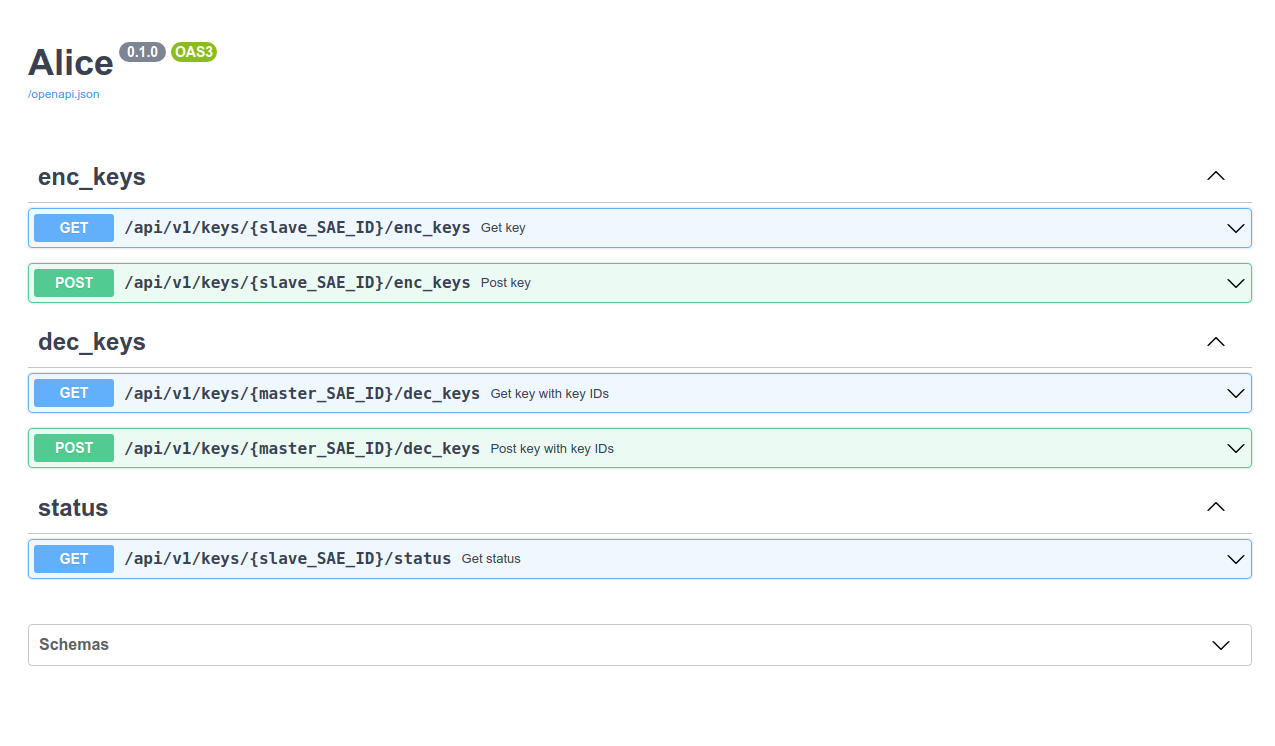
\includegraphics[width=1.0\textwidth]{Images/openapi.png}
    \caption{The web API interface made available by the KME thanks to FastAPI.}
    \label{fig:openapi}
\end{figure}

\begin{figure}[H]
    \centering
    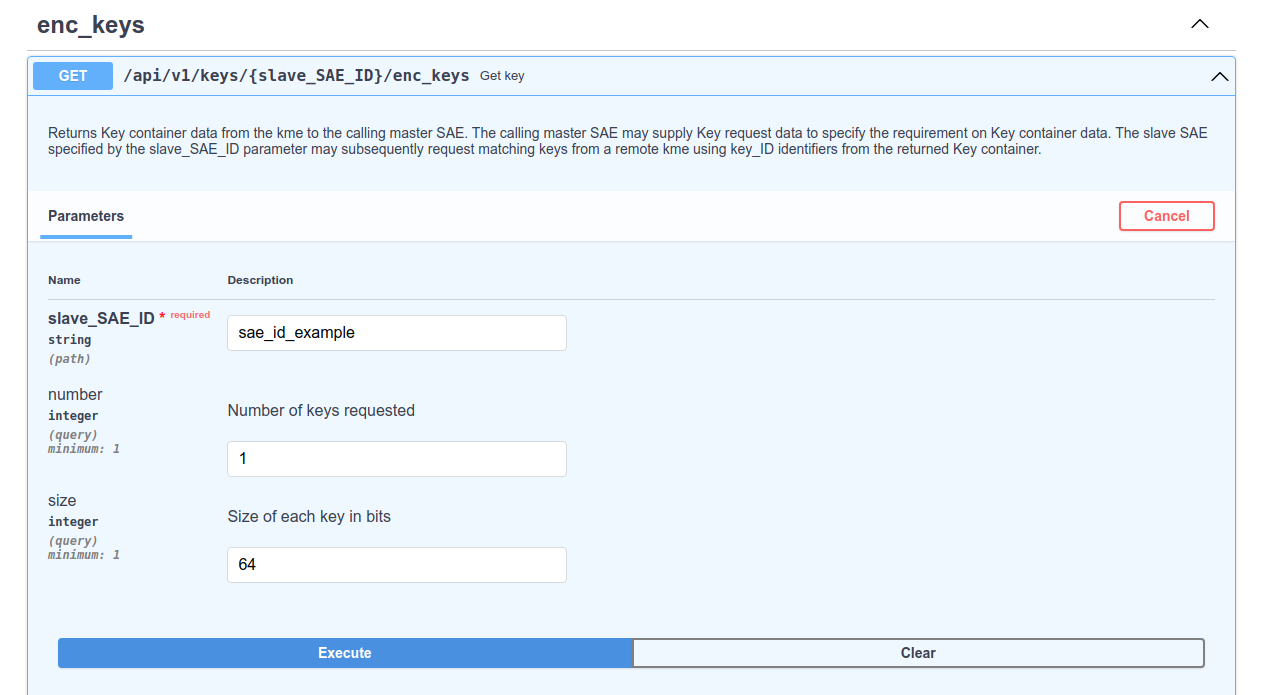
\includegraphics[width=1.0\textwidth]{Images/openapi_enc_keys.png}
    \caption{The simulation of a key generation request through the web API interface.}
    \label{fig:openapi_enc_keys}
\end{figure}

It is worth noting that FastAPI does not require explicit writing of these APIs: they are automatically created starting from the Python code written by the programmer. For example, here follows the signature of the Python function handling any HTTP GET request to the API \textit{/dec\_keys}:

\begin{minted}{python}
@router.get(path="/{master_SAE_ID}/dec_keys")
async def get_key_with_key_i_ds(
    master_SAE_ID: str,
    key_ID: UUID
) -> KeyContainer:
    ...
\end{minted}

FastAPI knows that the function is handling the API route \textit{/dec\_keys} thanks to the first line of code specifying the handled URL path. Then, FastAPI can retrieve the URL parameters required because they are the exact parameters of the Python function defined above. Moreover, FastAPI knows the JSON data format of the HTTP response body because it is of the same type specified as a return value for the Python function. For more information about how FastAPI can map Python functions to OpenAPI specifications, please refer to FastAPI documentation.

\section{Different modes of execution}
By default, the KME is started in "development mode": this is the environment used by the programmer while writing software. When the programmer wants to test the functioning of the project, it enters the so-called "testing mode". Then, the KME can be executed in "production mode" when the software is ready to be delivered. The choice of one environment changes some values of the configuration files. For example, the databases used in testing mode are not the same used in production mode. In Linux-based operating systems, it is possible to set the environment mode with the command:

\begin{minted}{bash}
export env=test
\end{minted}

Where the word "test" stands for "testing environment". Replace "test" with "dev" for explicitly activating the development environment; replace it with the word "prod" for activating the production environment. The same behavior can be achieved on the Windows command line with the command:

\begin{minted}{bash}
set env=test
\end{minted}

\section{The configuration file}
The project contains a configuration file that specifies important parameters relative to the KME behavior at runtime. Here follows a list of the main configuration parameters, whose overview may help to understand the way the different parts of the KME interact with each other:

\begin{itemize}
    \item KME\_ID: the ID of the KME. There is no standard way to specify the ID of a Key Management System. Therefore, we decided to call the two KMEs connected through the same quantum channel "Alice" and "Bob" in this project.
    \item HOST: the IP address \cite{ip} where the KME will run. By default, its value is "localhost", the network interface used to access network services running on the same host of the KME.
    \item PORT: the TCP port  \cite{tcp} where the KME will be listening to requests from SAEs.
    \item QC\_HOST: the IP address where the KME will be listening for new blocks coming from the quantum channel. By default, its value is also "localhost".
    \item QC\_PORT: the TCP port where the KME will be waiting for new blocks from the quantum channel.
    \item COMPANION\_URL: the URL where the cooperating KME is reachable. For example, suppose Alice is listening on "http://localhost:5000," and Bob is listening on "http://localhost:3000". In that case, Alice will have stored the listening URL of Bob, and vice versa.
    \item DEBUG: a Boolean flag whose value is True if debugging features enable is desired. When the KME is run in testing or development mode, this flag is set to True; it is set to False when in development mode.
    \item TESTING: a Boolean flag whose value depends on the running mode of the KME. In particular, it is True when the KME is run in testing mode, False otherwise. For more information about the testing mode, please see \ref{testing}.
\end{itemize}

\section{Quantum Channel Simulator}
\label{kme:qcs}

The implemented KME can communicate with Quantum Channels following the rules described in \ref{kme:qc}. However, working on the implementation of the KME, it was not always possible to communicate with the Quantum Channel in Politecnico di Milano. So, a piece of software simulating the behavior of a quantum channel was needed. Therefore, a Quantum Channel Simulator was implemented. This Quantum Channel Simulator does not provide the security strengths of a real Quantum Channel, and it is not intended for production purposes. However, it is convenient for testing and development environments. In order to start the Quantum Channel Simulator, the following command must be executed:

\begin{minted}{bash}
poetry run python -m qcs
\end{minted}

After starting the Quantum Channel Simulator, the KMEs connected will start receiving blocks. Therefore, they will be able to generate keys and perform all other tasks for which they were created.

As already mentioned, the material contained inside the blocks produced by the simulator is not the result of a Quantum Key Distribution Protocol. They are produced exploiting the function \textit{getrandbits()}, that is a function of the Python module called \textit{random}. Here follows the implementation of the function \textit{get\_random\_bits}, which is the core of the simulation of the generation of random bits:

\begin{minted}{python}
def get_random_bits() -> tuple[int, ...]:
    from random import getrandbits, randint

    # Generate a number of random bytes btw [lb, ub].
    lb, ub = 1000, 2000
    return tuple(getrandbits(8) for _ in range(randint(lb, ub)))
\end{minted}

The above Python code produces a pseudo-random number of pseudo-random bytes. The randomness depends on the internal implementation of the Python module \textit{random}, which is not based on QKD. So, once again, it is essential to notice that this simulator should not be exploited in an actual use case scenario.

Also, the number of bytes returned by the function is not deterministic. It is a value established by the function \textit{randint()}, that is also part of the Python module \textit{random}. This implementation choice aims at reproducing the behavior of a QKD protocol, which cannot determine the length of the block material \textit{a priori}, as discussed in \ref{kme:keys_vs_blocks}.

\section{Testing}
\label{testing}

When writing a software project, it is essential to write tests that are pieces of code intended to check that a given functionality is working as expected, despite the project's growth. Without a valid test suite, it is possible to modify part of the code introducing unexpected bugs.

Here, we exploited a Python test suite called \textit{pytest}. Thanks to \textit{pytest}, it is possible to execute all the tests written for the KME altogether with a single command:

\begin{minted}{bash}
poetry run pytest
\end{minted}

When the above command is executed, \textit{pytest} looks for all the files whose names start with the word "test". Then, inside such files, it looks for functions starting with the same prefix and executes them. This approach makes it easy to automate the testing phase. Each time the project is updated, it is possible to check the behavior of the KME executing the above command.

This KME implementation passes all the fifteen tests written for it. It is possible to read all the tests written for the KME inside the "tests" folder of the project.

\begin{figure}[H]
    \centering
    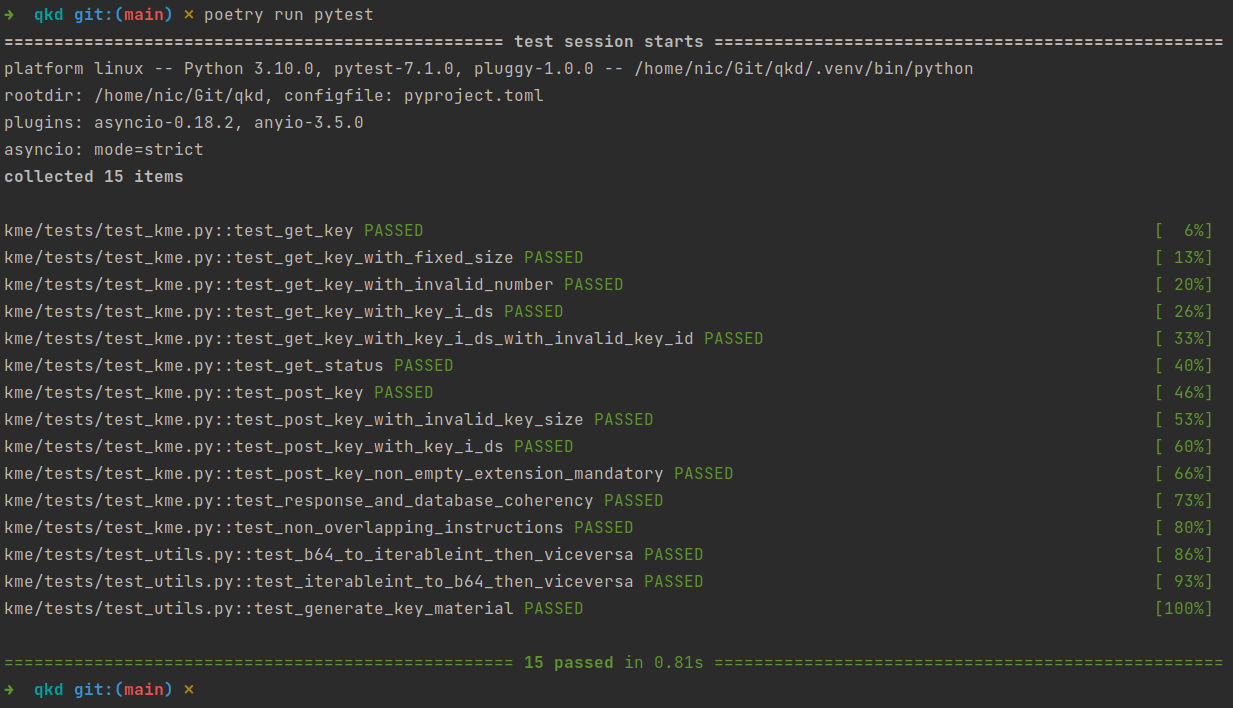
\includegraphics[width=1.0\textwidth]{Images/pytest.png}
    \caption{The result of the execution of the test suite with pytest.}
    \label{fig:pytest}
\end{figure}

Another critical aspect of testing is code coverage. The executed test suite should involve all the lines of code of the project. However, this is not sufficient to ensure that the project is free from bugs. In order to test the code coverage, this project exploits another Python package called "coverage". In order to run a test coverage, it is enough to execute the following command:

\begin{minted}{bash}
poetry run coverage report
\end{minted}

At the time of writing, the coverage of the project is near 94\%, which is considered a fair coverage value.

\begin{figure}[H]
    \centering
    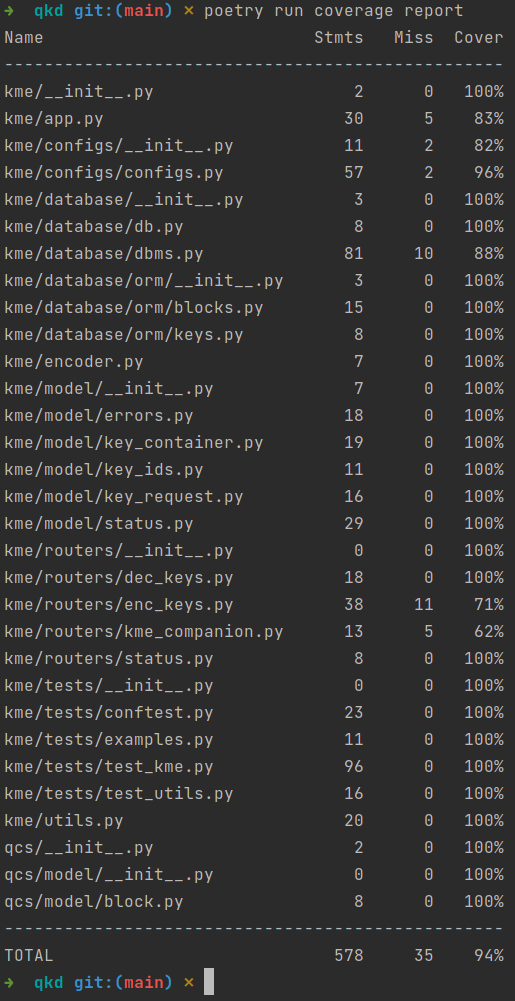
\includegraphics[width=0.6\textwidth]{Images/coverage.png}
    \caption{The result of the execution of the coverage test.}
    \label{fig:coverage}
\end{figure}

\section{Asynchronicity}
A notable feature of this implementation of a Key Management Entity is its ability to handle multiple Secure Application Entities requests concurrently. A great effort has been spent to make this KME implementation able to manage requests asynchronously. The concept of asynchronicity can be well explained through an example use case. 
Consider two Secure Application Entities, SAE A and SAE B, making requests to the same Key Management Entity. SAE A asks to create 50 new keys that are 2048 bits long. Then, SAE B asks for the key associated to the UUID 5835e93e-5250-4a85-b5d0-20ddf10e2f12. Notice that the request of SAE A requires an effort that is significantly greater than the one required for handling the request by SAE B. In a synchronous context, SAE B would receive the response to its "light" request only after SAE A has received its response. Instead, SAE B may receive its response before SAE A in this asynchronous context.
Moreover, suppose other Secure Application Entities send requests to the KME that are relatively easy to manage. In that case, the KME may send them a response while working on the answer to SAE A. The asynchronous management of the requests may significantly improve the performance of the KME.

The implementation of these features relies on Python's syntax, which allows defining a function with a signature that starts with the keyword \textit{async}. Lines of code that can be executed asynchronously inside an async function starts with the keyword \textit{await}. Indeed, while the Python interpreter is waiting for the result of an asynchronous request, it can devote time to handling other requests. For example, consider the following lines of code:

\begin{minted}{python}
async def generate(size: int) -> Key:
    key_id = uuid4()
    key_material, instructions = await generate_key_material(size)

    await orm.Key.objects.create(key_id, instructions)

    return Key(key_id, key_material)
\end{minted}

The one above is the function for creating one new key of fixed length. The second line of the function calls another function, \textit{generate\_key\_material}, devoted to the creation of key material, starting from blocks. This operation may be expensive in terms of time. So, while waiting for its termination, Python handles other requests. Finally, when the new key is generated, the third line of code is executed: it stores the instructions of the newly-generated key into the shared database. Also, this operation may be expensive, so it is "awaited". In the end, the new key is returned to the calling function.

One crucial aspect of asynchronicity is access to the databases. Indeed, making queries to a database is an expensive operation. This project uses a Python package called "orm", which allows making asynchronous queries to the database. Queries that only want to read the content of the database can be managed concurrently without worrying about the order they are made. Instead, two concurrent accesses to the local database for retrieving a block fragment are dangerous: they should not receive the same block fragment as a response. This behavior would lead to the exploitation of the same block material to build distinct keys, which is not the desired effect. Therefore, when one function requests a block fragment, that fragment is popped up from the database and is returned only to that function. When the function ends the exploitation of the block, if there are unexploited block material bits left, it re-inserts the updated block fragment inside the database.

The entire implementation of this KME is asynchronous: the management of requests to the API, the access to the databases, and the testing phase. This feature leads to the performance benefits previously described.
\chapter{Experimental results}
\label{ch:chapter_4}%

We introduced the Key Management Entity in the previous chapters and described its implementation details. Here, we will show three use cases to demonstrate that our implementation of the KME works as expected.

In all the following experiments, we will not use the Quantum Channel Simulator described in \ref{kme:qcs} and exploited during the development process. Instead, the KMEs will receive blocks from the Quantum Channel maintained in Politecnico di Milano. The goal is to provide examples of operations of the KME in situations that are as close to actual use case scenarios as possible. The details about how to boot and configure the quantum channel are out of the scope of this document.

All the experiments require the boot of the quantum channel and two cooperating KMEs, which are two KMEs linked to the different endpoints of the same quantum channel. We will refer to these KMEs as Alice and Bob to distinguish them.

We boot one KME with ID "Alice" on our machine. It listens to new blocks from the Quantum Channel on TCP port 9998 and listens to requests from the API on TCP port 5000. These settings must be defined before booting the KME, modifying its configuration file. When  everything is ready, it is possible to start Alice with the command:

\begin{minted}{bash}
poetry run python -m kme
\end{minted}

Then, we boot another KME with ID "Bob" on the same machine. So, Alice and Bob are both executing on localhost. Bob listens to new blocks from the Quantum Channel on TCP port 9999 and listens to requests from the API on TCP port 3000. Now, it is possible to start Bob with the command above.

There should not be an overlap between TCP ports because Alice and Bob are running on the same machine, so this would lead to undesired network conflicts.

Alice and Bob receive blocks from the quantum channel and store them locally during the execution. Chapter 2 deepened the details of the cooperation between the two KMEs and their communication with the quantum channel.

In the following figures, Alice and Bob have been booted and are receiving the very same blocks from the quantum channel.

\begin{figure}[H]
    \centering
    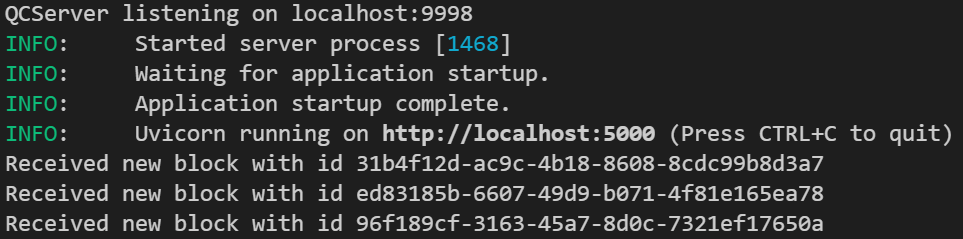
\includegraphics[width=0.8\textwidth]{Images/alice.png}
    \caption{Alice listening on TCP port 5000.}
    \label{fig:alice}
\end{figure}

\begin{figure}[H]
    \centering
    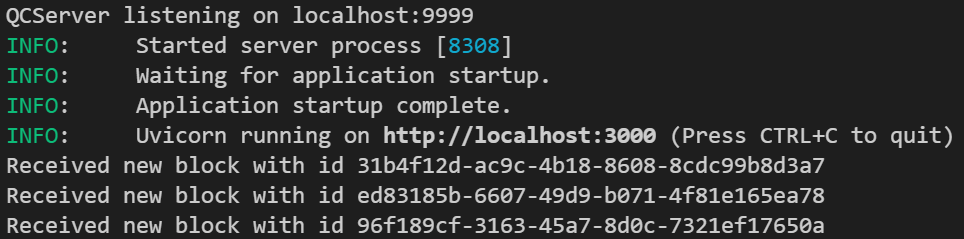
\includegraphics[width=0.8\textwidth]{Images/bob.png}
    \caption{Bob listening on TCP port 3000.}
    \label{fig:bob}
\end{figure}

\section{First experiment: successful generation of a new key}
We want to exhibit regular communication between Alice and Bob in this first experiment. In particular, we request to Alice the generation of one key of length 256 bits. Alice responds with a key containing material of length 256 and a UUID.
Then, we request Bob to retrieve the key associated with the given UUID. If Bob responds with the very same key produced by Alice, then the experiment is successful.

Let us start the experiment. We request the generation of a new key of length 256 to Alice. The following is our HTTP request:

\begin{minted}{bash}
http://localhost:5000/api/v1/keys/BobApp/enc_keys?number=1&size=256
\end{minted}

Alice answers with an HTTP response having the following Key Container object as body:

\begin{minted}{json}
{
  "keys": [{
      "key_ID": "5df98759-6705-4de6-8f76-9c37adba7d82",
      "key": "/otfMnKVYI57Km2IA2Bs1jZAi5e9bBtli/7j5Vn1MQw="
    }]
}
\end{minted}

Now, we send Bob an HTTP GET request containing the above key\_ID, that is, the UUID of the key generated by Alice. Here is our HTTP request to Bob:

\begin{minted}{bash}
http://localhost:3000/api/v1/keys/AliceApp/
dec_keys?key_ID=5df98759-6705-4de6-8f76-9c37adba7d82
\end{minted}

The following is Bob's answer, with HTTP status code 200:
\begin{minted}{json}
{ "keys": [{
      "key_ID": "5df98759-6705-4de6-8f76-9c37adba7d82",
      "key": "/otfMnKVYI57Km2IA2Bs1jZAi5e9bBtli/7j5Vn1MQw="
    }]
}
\end{minted}

Bob returns the same key produced by Alice, confirming a successful communication between them.

\section{Second experiment: failure retrieving a key without the needed blocks}
In this second experiment, we focus on the communication between Alice and Bob again. Now, however, we analyze a situation where an error occurs. In particular, after Alice gives us one key with a material of length 256, we manually delete all the local database entries where Bob stores the blocks received from the Quantum Channel. When we ask Bob to retrieve the key associated with the given UUID, it cannot re-build that key. In fact, after reading from the shared database the instructions about how to re-build the key, Bob does not find the necessary blocks in its local database of blocks. This situation forces Bob to respond to our retrieval request with an error message.

Let us start the experiment. We request the generation of a new key of length 256 to Alice. The following is our HTTP request:

\begin{minted}{bash}
http://localhost:5000/api/v1/keys/BobApp/enc_keys?number=1&size=256
\end{minted}

Alice answers with an HTTP response having the following Key Container object as body:

\begin{minted}{json}
{ "keys": [{
      "key_ID": "4610bc87-271a-4fd2-a01c-4c8fc5498ed5",
      "key": "2WCmDSuiE1g7heV2rlhSgt2qflgC/NGUqmJcAM5FiD0="
    }]
}
\end{minted}

Now, we manually delete all the blocks from Bob's local DB. Asking for the key produced by Alice, we expect to get an HTTP error response. Here is our HTTP request to Bob:

\begin{minted}{bash}
http://localhost:3000/api/v1/keys/AliceApp/
dec_keys?key_ID=4610bc87-271a-4fd2-a01c-4c8fc5498ed5
\end{minted}

The following is Bob's answer, with HTTP status code 400:

\begin{minted}{json}
{ "message": "One or more keys specified are not found on KME" }
\end{minted}

The message that the KME returns to the calling SAE is generic and points out that it could not re-build the requested key. In Bob's logging console, we can also find the following message:

\begin{minted}{bash}
ERROR: Block with UUID c3c8a268-9a26-41d4-ae77-105b0dd360fb not found
\end{minted}

This message confirms that the error was produced by the inability of KME Bob to retrieve a block pointed out in the instructions for re-building the key with the given UUID. So, our experiment has been successful.

\label{ch4:exp3}
\section{Third experiment: successful cooperation between three KMEs}
We consider a more sophisticated situation in the third experiment than previously described. Up to now, we have focused on two cooperating KMEs linked to the same quantum channel. Each KME received blocks from the same quantum channel. However, our implementation of a KME can handle blocks coming from multiple quantum channels. Each quantum channel is identified by a UUID, which is embedded into the block when sent to the KME. Therefore, the fields of a block sent to the KME are:

\begin{itemize}
 	\item \textit{block\_id}: the UUID of the block;
	\item \textit{material}: the block material;
	\item \textit{timestamp}: the timestamp of the block;
	\item \textit{link\_id}: the UUID of the quantum channel that produced this block.
\end{itemize}

One master SAE wants to request the generation of keys produced from blocks of a particular quantum channel. In order to do so, it has to exploit the HTTP POST request \textit{enc\_keys}, specifying "link\_id" as an "extension mandatory" parameter. For more details about the structure of this API interface, please see \ref{kme:key_gen}.

By now, we manually provide the UUID of the quantum channel. In the last chapter of this document, we will see one future development purpose for automating the process.

So, in this experiment, we will consider two quantum channels:
\begin{itemize}
    \item QC\_A, associated with the UUID de2e6bbe-4897-40df-8532-b7425a6f57d9;
    \item QC\_B, associated with the UUID 231656cb-d062-4897-bb11-8d3a551e720c.
\end{itemize}

Then, we will consider three KMEs:
\begin{itemize}
    \item Alice, which receives blocks from both QC\_A and QC\_B;
    \item Bob\_A, which receives blocks only from QC\_A;
    \item Bob\_B, which receives blocks only from QC\_B;
\end{itemize}

Therefore, Alice and Bob\_A cooperate through the QC\_A, while Alice and Bob\_B cooperate through the QC\_B. Bob\_A and Bob\_B do not cooperate.

Alice and Bob\_A will use the same port as in the previous experiment. Bob\_B, instead, will listen for new blocks coming from QC\_B on TCP port 9997 and listen to API requests on TCP port 8000.

\begin{figure}[H]
    \centering
    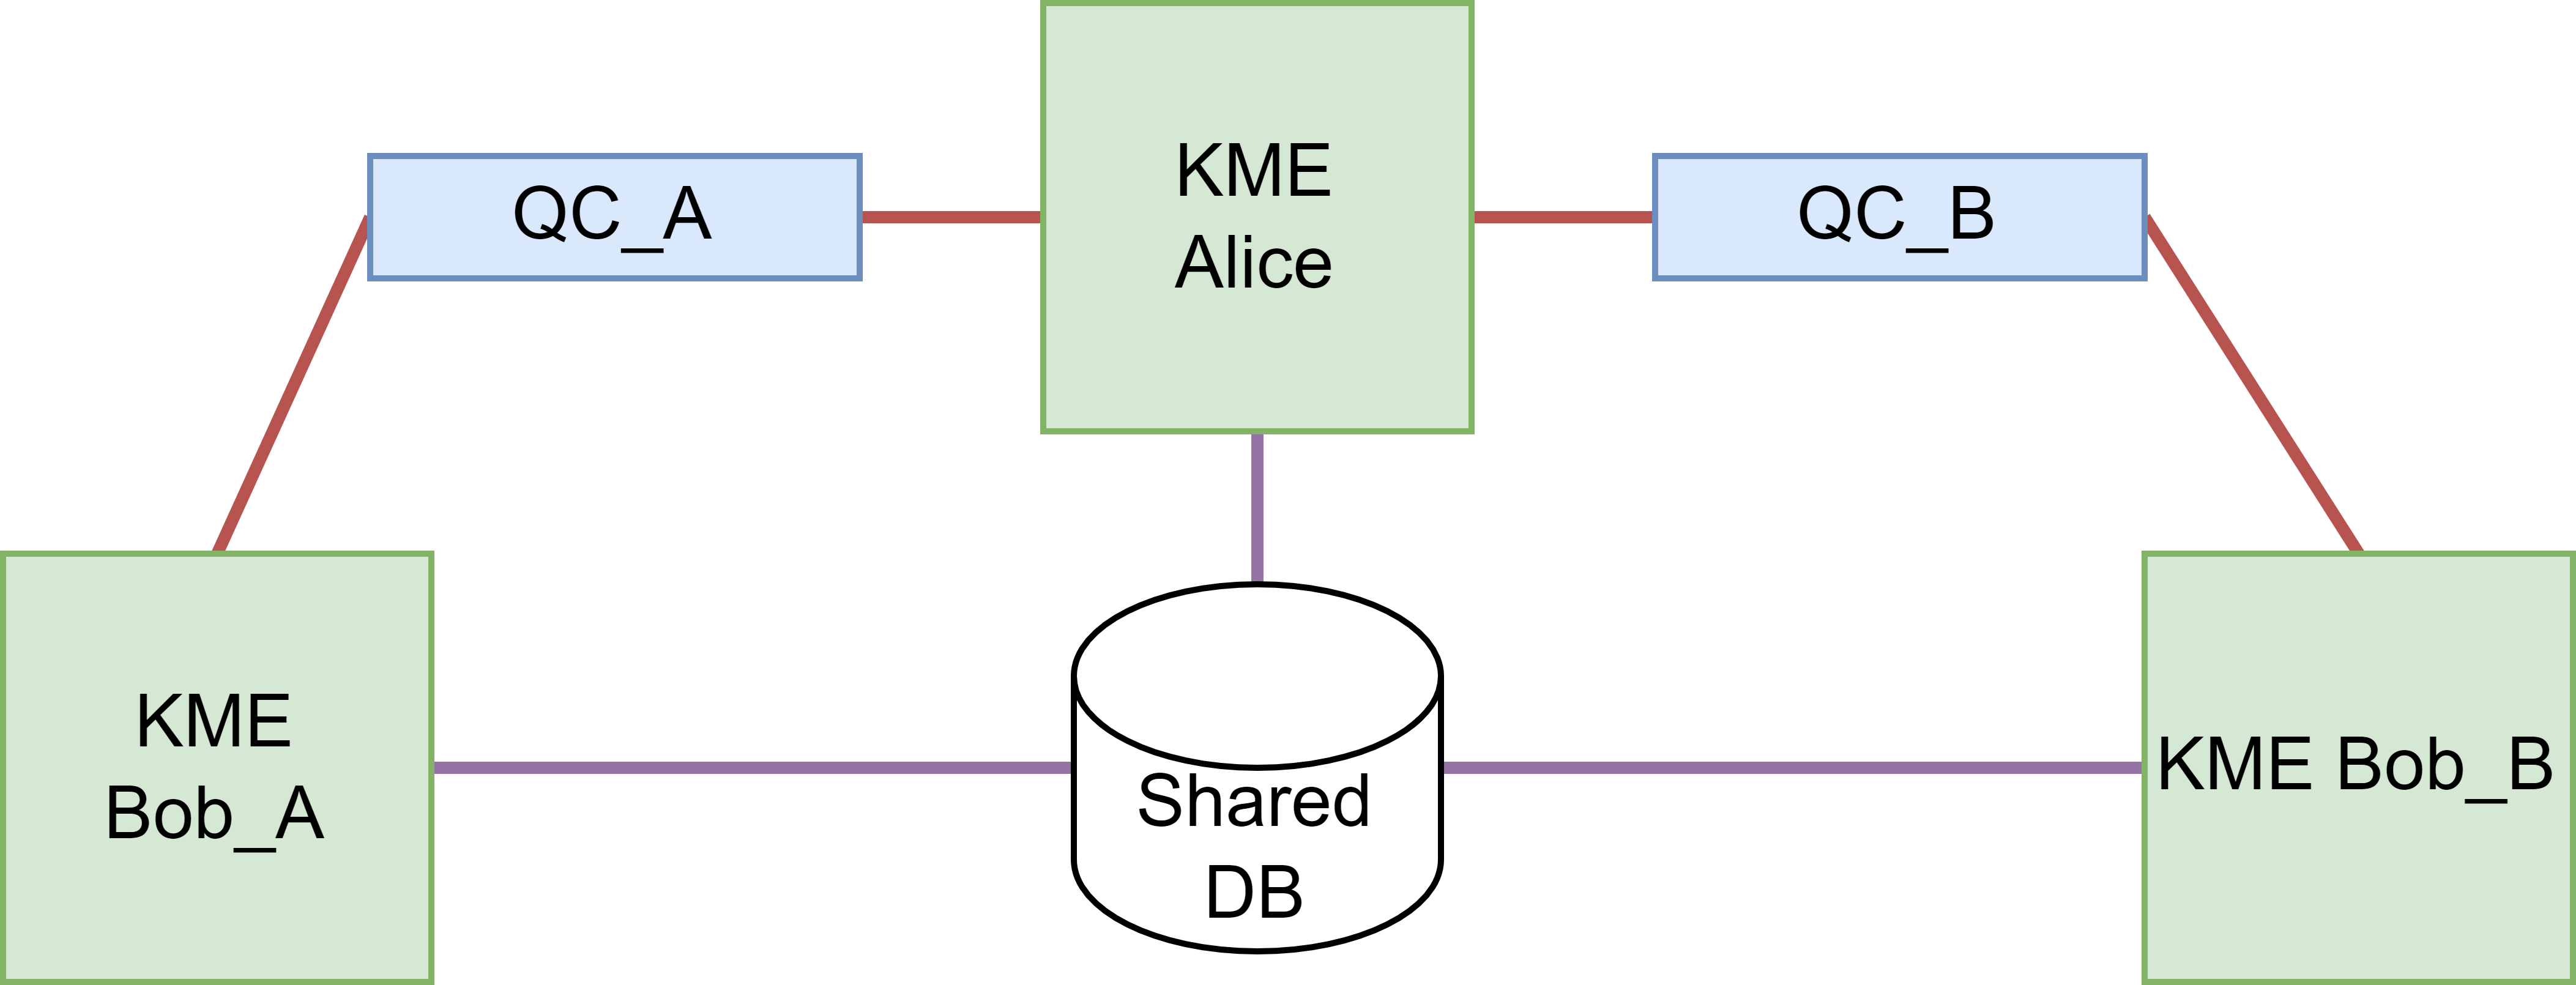
\includegraphics[width=1.0\textwidth]{Images/Third experiment.png}
    \caption{The topology of the third experiment.}
    \label{fig:third_exp}
\end{figure}

In this experiment, we will request Alice to generate a new key of length 256 bits exploiting blocks coming from the QC\_A. Then, we will request Bob\_A to retrieve the new key. Bob\_A cooperates with Alice through the QC\_A, so we expect to receive a successful HTTP response. Then, we will request Bob\_B to retrieve the very same key. However, Bob\_B does not cooperate with Alice through QC\_A, so we expect to receive an HTTP error response. Indeed, Bob\_B does not receive blocks from QC\_A, so it cannot find the blocks listed in the instructions shared between all the KMEs through the shared DB.

Let the experiment begin.
First, we request Alice to generate a new key of length 256 bits manipulating blocks from QC\_A. In order to do so, we exploit the HTTP POST request method \textit{enc\_keys}. The following is the request URL of the HTTP request:

\begin{minted}{bash}
http://localhost:5000/api/v1/keys/Bob_A_App/enc_keys
\end{minted}

While the following is the body of the HTTP request:
\begin{minted}{json}
{
  "number": 1,
  "size": 256,
  "extension_mandatory": [
    {"link_id": "de2e6bbe-4897-40df-8532-b7425a6f57d9"}
  ]
}
\end{minted}

Alice uses the blocks produced by the quantum channel associated with the link\_id specified in the request body. Then, it sends us an HTTP response with status code 200 and the following body, which is a Key Container object with the newly generated key:
\begin{minted}{json}
{ "keys": [{
      "key_ID": "afe2b30e-206b-410c-ab51-63d2d7726a12",
      "key": "eVzqbEODx8fxkQVnGgEys4aztzat94nP96SCcYVZSHE="
    }]
}
\end{minted}

Now, we use the key\_ID of the newly-generated key for asking Bob\_A and Bob\_B to re-build that key.

The HTTP request we send to them is the same:

\begin{minted}{bash}
http://localhost:3000/api/v1/keys/AliceApp/
dec_keys?key_ID=afe2b30e-206b-410c-ab51-63d2d7726a12
\end{minted}

However, the HTTP responses are different, as we expected. The HTTP response of Bob\_A has status code 200, and its body contains the same key returned by Alice:
\begin{minted}{json}
{ "keys": [{
      "key_ID": "afe2b30e-206b-410c-ab51-63d2d7726a12",
      "key": "eVzqbEODx8fxkQVnGgEys4aztzat94nP96SCcYVZSHE="
    }]
}
\end{minted}

Bob\_B's HTTP response, instead, has status code 400, and it does not contain the key associated with the given UUID. We repeat that this behavior is the one desired. Bob\_B does not know the blocks generated by the QC\_A: only Alice and Bob\_A know them. The public instructions on how to re-build the key with UUID afe2b30e-206b-410c-ab51-63d2d7726a12 are not enough to know the key material associated with that UUID. The shared DB does not compromise the security assumptions of the system in any way.
\chapter{Conclusions and future developments}
\label{ch:conclusions}%

Quantum Key Distribution (QKD) is an information-theoretic secure protocol that solves the computational problems of classical key-exchange algorithms. However, exploiting QKD, the secret sequences of bits produced by a Quantum Channel, which we call blocks, have non-deterministic lengths. So, they cannot be delivered directly to Secure Application Entities (SAEs), requiring fixed-sized keys to encrypt messages.

The Key Management Entity (KME) is the middleware that builds fixed-sized keys, starting from the blocks produced by a Quantum Channel. Moreover, cooperating KMEs supervise the distribution of generated keys to one or multiple Secure Application Entities.

This thesis work focused on implementing a Key Management Entity and exploring its relationship with Quantum Channels, SAEs, and other KMEs. First, we made the KME communicate with the Quantum Channel realized in Politecnico di Milano. Then, we implemented the KME and SAEs interface following the standard ETSI GS QKD 014. Finally, we showed some actual use case scenarios of the Key Management Entity cooperating with other KMEs.

Our implementation of the KME can handle multiple requests from SAEs asynchronously. Moreover, it manages the blocks produced by the Quantum Channel so that its quantum devices do not have to devote resources to address these blocks. Finally, the KME can communicate with multiple Quantum Channels, receiving their blocks and handling SAE's requests for keys produced by exploiting blocks of a specific QC.

However, the development process of the KME is not done. First, the KME should define an authentication mechanism for SAEs connecting to it. Then, it should improve its capabilities of managing changes in the topology of the underlying network of Quantum Channels. Chapter 4 showed an example where one KME handles blocks from two different Quantum Channels. However, we had to manually communicate the UUID of the Quantum Channel for each request to the KME.

The solution to these problems may be a centralized entity called an SDN controller, whose implementation is described in standard ETSI GS QKD 015 \cite{etsi015}. The SDN controller would communicate with all the entities of a QKD network - i.e., the Quantum Channels, the KMEs, the SAEs - ensuring coherent and automatic management of the key delivery process. Therefore, a notable improvement for the KME would be implementing a communication interface with the SDN controller. Thanks to this feature, the SAEs' authentication and the configuration parameters' definition would be managed automatically inside the Quantum Key Network.

%-------------------------------------------------------------------------
%	BIBLIOGRAPHY
%-------------------------------------------------------------------------

\addtocontents{toc}{\vspace{2em}} % Add a gap in the Contents, for aesthetics
\bibliography{bibliography} % The references information are stored in the file named "bibliography.bib"

%-------------------------------------------------------------------------
%	APPENDICES
%-------------------------------------------------------------------------

\cleardoublepage
\addtocontents{toc}{\vspace{2em}} % Add a gap in the Contents, for aesthetics
\appendix

% LIST OF FIGURES
\listoffigures

\cleardoublepage

\end{document}
